\documentclass[DIV=calc, paper=a4, fontsize=10pt, twocolumn]{article}
\usepackage{graphicx}
\usepackage{color}
\usepackage{amsmath}
\usepackage{float}
\usepackage{caption,lipsum}
\usepackage{amssymb}
\usepackage{subcaption}
\usepackage[colorlinks=true]{hyperref}
\usepackage{geometry}
\usepackage{multirow}

\usepackage{tikz}
\usetikzlibrary{positioning}
\usepackage{xcolor}
\usetikzlibrary{decorations.text}
\usetikzlibrary{shapes.geometric}

\tikzset{base/.style={draw, align=center, minimum height=4ex},
	test1/.style={base, diamond, aspect=2, text width=5em, inner sep=5pt},
	test2/.style={base, diamond, aspect=2, text width=5em, inner sep=-4pt}
}

\geometry{a4paper,scale=0.8}
\title{CE4042 Assignment 2\\
	\large Gender-Age-Race Classification}
\author{Hu Kairui, Hu Siyuan, Hu Tianrun}
\date{\today}

\begin{document}
	\maketitle
	\section{Introduction}
	
	Gender, race classification and age estimation based on face images are three common tasks conducted by human eyes on a daily basis, and they also form an important field that has been long researched by computer vision scientists. Gender race classification and age estimation have a broad application in real world scenarios, such as security and e-commerce, to name a few. Therefore, a high performance model tackling these problems is of great significance. However, different from face detection and recognition tasks, accurate gender race classification and age estimation involve multiple challenges. Firstly, the gradual aging process results in similar facial appearances corresponding to similar ages, while large age differences lead to notably different facial appearances. Secondly, most of the datasets available are small and imbalanced, which may introduce bias to experiment results. Lastly, the facial appearance variation pattern due to aging is complex and may be caused by multiple intrinsic and extrinsic factors, such as race, gender and lifestyle. Gender age classification and age estimation can be formulated into the following problem, given a latent embedding of the face images $\mathcal{X}$, a gender as one of $\{g\}_1^c$ and an race as one of $\{r\}_1^c$ is classified corresponding to an image $x$, $g_i\in\mathbb{Z}^+$, $r_i\in\mathbb{Z}^+$, $x\in\mathcal{X}$. It is worth noting that age estimation are commonly formulated into a scalar regression problem, where age is represented as $a\in\mathbb{R}^+$ that is continual. However, in our setting age is represented as $a\in\mathbb{Z}^+$ that corresponds to discrete age groups. This is to utilize datasets with face images not labeled with specific age values but age groups. While for datasets whose images are labeled with specific age values, the interval between age groups would be set to 1, which will convert the classification problem equivalent to the regression problem. The successful use of Deep Learning-based methods in computer vision tasks has paved the path for deriving end-to-end gender race classification and age estimation models, and Convolutional Neural Networks are the most representative ones. CNN-based methods learn local features based on the age differences as a metric measure. 
	\begin{figure}[t]
		\centering
		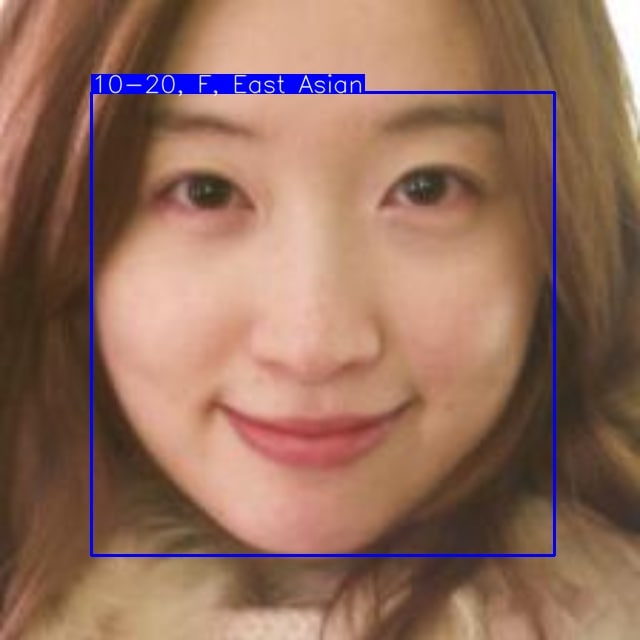
\includegraphics[width=0.9\linewidth]{"./imgs/result_2_F_East_Asian_9220.jpg"}
		\caption{Example of prediction}
		\label{fig:result2meast-asian9220}
	\end{figure}
	
	In this work we first proposed an end-to-end gender-age-race ternary classification model as a baseline. Afterwards, we proposed a Gender-specific Fusion model to harness the gender-specific information and further improve the performance, depicted in Fig. \textcolor{red}{1}. Firstly, we looked into the model performance degradation problem caused by training on unbalanced datasets, and conducted experiments to reveal its impact. Secondly, with an appropriate dataset selection as the starting point, we employed the idea of Transfer Learning by using a pre-trained model trained on ImageNet dataset, and performed downstream fine-tuning on our face attribute classification datasets. This can help leverage the strong capacity of large-scale models and save computing costs by skipping early epochs. Thirdly, to verify our intuitive insight that age-race prediction of different genders tends to exhibit different patterns, for example, females are more effective at hiding their ages due to social commentaries, we employed a gender-specific stacked fusion model that the gender is classified first, then the image is fed into different gender-specific classifiers to do the further predictions on age and race. 
	
	In particular, we proposed the following ideas:
	
	$\bullet$ We proposed an end-to-end gender-age-race classification solution based on a ResNet pre-trained model as the foundation.
	
	$\bullet$ We proposed a Gender-specific Fusion model with a two-stage architecture for the gender classification and the age-race estimation sub-tasks, considering the gender-specific information. 
	
	$\bullet$ Our proposed fusion model achieves a higher accuracy than the original end-to-end models when applied to contemporary face image datasets UTKface and FairFace. 
	
	\section{Related Work}
	Despite the inherent challenges brought on by the different facial aging characteristics, and variations between races, gender, and lifestyles, human observers can reliably estimate age based on the face on a daily basis. The fundamental work of Buolamwini and Gebru \cite{Guo2010HumanAE} showed the significance of race and gender in face analysis and recognition, and it is particularly interesting. Guo and Mu \cite{pmlr-v81-buolamwini18a} developed a two-step process in which the age is individually estimated for each gender and race group after first classifying gender and race.
	
	\subsection{Face Attribute Recognition} 
	The task of classifying different human characteristics from facial appearance, such as gender, race, age, emotions, expressions, or other facial aspects, is known as face attribute recognition. Multiple computer vision systems have included face attribute recognition as a minor component. For instance, Kumar et al. \cite{kumar2011describable} employed features for face verification that included facial characteristics that characterize individual traits, such as gender, race, hair style, expressions, and accessories. Additionally, attributes are frequently used to re-identify people in photos or videos by fusing characteristics of the human face and body \cite{layne2012person, li2014clothing, su2017multi}, which is particularly successful when faces are obscured or too small. These systems can be used for security purposes such as CCTV monitoring or electronic device authentication (like unlocking cellphones) \cite{grgic2011scface}. Face attribute recognition is frequently used for demographic research in social science and marketing, which aims to determine how social actions of people relate to their backgrounds in terms of demographics. Social scientists, who traditionally did not utilize photos, have started to use images of people to infer their demographic traits and evaluate their activities in many research using commercial services and off-the-shelf techniques \cite{amos2016openface, baltrusaitis2018openface}. Examples include demographic studies of social media users that use their images \cite{chakraborty2017makes, reis2017demographics, wang2017polarized, won2017protest, xi2020understanding}.
	
	\subsection{Transfer Learning} 
	
	Deep neural network architectures such as convolutional neural networks (CNNs) and more recently transformers have achieved many successes in image classification tasks. It has been consistently shown that these models work best when big models can be trained and there is an abundance of labeled data available for the task \cite{kolesnikov2020big, mahajan2018exploring, ngiam2018domain}. However, there are numerous situations in real life where the need for a lot of training data cannot be satisfied. Among them are:
	
	$\bullet$ Insufficient data due to privacy concerns or the rarity of the data. For instance, because to the rarity of the examples themselves as well as privacy considerations, training data for novel and rare disease identification tasks in the medical area is scarce. 
	
	$\bullet$ The cost of data collection and/or labeling is prohibitive. For instance, only highly qualified subject-matter specialists can perform labeling.
	
	We may want to learn from a limited number of training instances for a variety of additional reasons as well: 
	
	$\bullet$ From a cognitive science perspective, it is intriguing to make an effort to emulate the human capacity to learn general concepts from a sparse sample size. 
	
	$\bullet$ Compute resource limitations could make it difficult to train a big model from random initialization with big data. Consider environmental issues \cite{strubell2019energy}. 
	
	Transfer learning frequently significantly improves performance in all of these instances. In this paradigm, the trained weights are utilized to initialize a model for the target task after the model has been trained on a similar dataset and task for which additional data are available. The dataset must be sufficiently connected and best practice techniques must be applied for this process to boost performance rather than degrade it.
	
	\section{Method}
	\subsection{ResNet}
	For our gender, age, and race classification task, we used ResNet, a deep residual learning framework, as the pre-trained model. ResNet\cite{he2016deep} helps address the model degradation problem by enabling stacked layers to fit a residual mapping. Mathematically, let the targeted underlying mapping be $H(x)$, then the stacked layers fit the mapping of $F(x): H(x)-x$. The original mapping becomes $F(x)+x$. Compared with the original mapping, it is easier to  learn the residual mapping. We can explain the learning mathematically. The residual unit can be denoted as: 
	$$
	y_l=h(x_l)+F(x_l, W_l),
	x_{l+1}=f(y_l)
	$$
	With $x_l$ and $x_{l+1}$ be the input and output of the $l$th residual unit. $F$ is the residual function indicating the learned residual, $h(x_l)=x_l$ denotes the identity mapping, and $f$ is the ReLU activation function. The feature we learn from layer $l$ to deeper layer $L$ is:
	$$
	x_L=x_l+\sum_{i=l}^{L-1}F(x_i, W_i)
	$$
	
	
Based on the chain rule, we can obtain the gradient:
	
	$$
	\begin{aligned}
		\frac{\partial loss}{\partial x_l} & = \frac{\partial loss}{\partial x_L}*\frac{\partial x_L}{\partial x_l} \\
		& = \frac{\partial loss}{\partial x_L}*(1+\frac{\partial}{\partial x_l}\sum_{i=l}^{L-1}F(x_i, W_i))
	\end{aligned}
	$$
	With $\frac{\partial loss}{\partial x_L}$ denoting the gradient of the loss function at L, 1 in parentheses indicates that the shortcut connection propagates the gradient losslessly, and the presence of 1 does not cause the gradient to vanish. Hence, residual learning will be easier.
	
	
	\subsection{Gender, Age, Race classification}
	We first perform the three classification tasks together with the pre-trained ResNet model. For the labeling purpose in training, we labeled the gender, age, and race as the corresponding natural numbers starting from 0. The model takes an input RGB image of size 224 x 224. It consists of the pre-trained ResNet and 3 additional parallel dense layers as classification heads for producing the corresponding 3 output labels. We select the output label with the SoftMax activation, which is defined below:
	$$
	\begin{aligned}
		\sigma(\boldsymbol{z})_i = \frac{e^{z_i}}{\sum_{j=1}^{K}e^{z_j}}
	\end{aligned}
	$$
	$$
	\begin{aligned}
		\text{for } i=1,...K \text{ and } \boldsymbol{z}=(z_1,...,z_K)\in\mathbb{R}^K
	\end{aligned}
	$$
	
	
	The cross-entropy loss function defined is used to optimize the classification model:
	 $$
	 \begin{aligned}
	 	L=-\frac{1}{m}\sum_{i=1}^{m}y_i*log(\hat{y_i})
	 \end{aligned}
	 $$
	
	The epoch for the training process is set to 30. In order to prevent overfitting, we implemented early stopping with a patience of 5. The model is optimized by the Adam optimizer, and we implemented learning rate decay as the number of epoch goes up. 
	
	
	The architecture of the model is shown in Figure \ref{fig:end-to-end}.

	\begin{figure}[t]
	\centering
	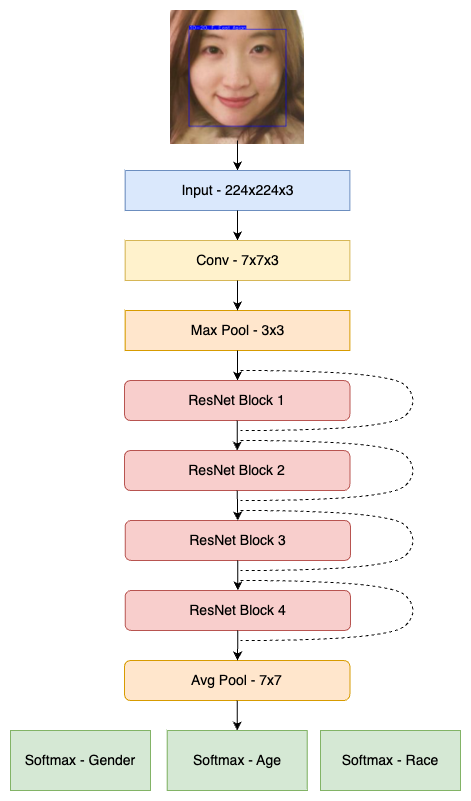
\includegraphics[width=0.9\linewidth]{imgs/original}
	\caption{End-to-end Model Architecture}
	\label{fig:end-to-end}
	\end{figure}
	
	\subsubsection{Transfer Learning}
	Transfer Learning refers to pre-training on large-scale general datasets and fine-tuning on small datasets according to the requirements of downstream tasks. Therefore, Transfer Learning can greatly benefit face image related tasks, as models can directly inherit the knowledge of human faces' basic representations from pre-trained models, thus time-consuming early epochs can be skipped. To leverage the advantages of pre-trained models, we employed multiple models well-trained on ImageNet as the foundation, as ImageNet contains rich image representation knowledge. Moreover, the original last layer is replaced by 3 parallel dense softmax classification heads, and a flatten layer is added as the penultimate layer to reshape the classification head input. After modifying the model architecture to adapt to the gender, age, race classification task, further fine-tuning on our face image datasets can be performed.
	
	\subsubsection{Dataset Augmentation}
	As complex network architectures are employed in our model design, dataset augmentation is of great importance to prevent overfitting on small datasets. To be specific, the augmentation pipeline is composed of random cropping, flipping and light adjustment, and each will be executed according to its configured probability. Image augmentation will be executed during data loading in each epoch, therefore, the original small datasets can be enriched to a great extent. It is worth noting that the training processes of two gender-specific classification models will employ more augmentation. As the original dataset will be split in half to train the gender-specific models, while they share the architecture of same depth with the end-to-end model which is trained on the entire dataset, more image augmentation is required for the gender-specific models to ensure that they are trained to the same extent as the end-to-end model to ensure fairness. 
	
	\subsection{Gender-specific Fusion Model}
	There are many difference features between men and women. To harness the gender-specific information in the classification tasks, we proposed a Gender-specific Fusion model consisting of two main modules. The first module is a gender classifier that classifies the input image into one of the two gender categories. The second module consists of two gender-specific classifiers, denoted as Male-classifier and Female-classifier. The Male classifier performs age and race predictions for the input images classified as male, and the Female-classifier performs age and race predictions for the female subjects. With this two-stage architecture, given an input image for the age-gender-race classification task, we can first classify its gender, after which we put this image into the Male or Female classifier to perform further predictions on age and race. 
	
	To effectively train the two gender-specific classifiers, we divided the training set into the male and female dataset based on the gender label. The Male classifier was solely trained on the male dataset, and the Female classifier was trained only on the female dataset. To establish a fair training setup, we performed data augmentation on the sub-datasets to ensure each of the two sub-datasets has the same number of data inputs as the original dataset, so that the two gender-specific classifiers can be trained on a dataset with the same size as the original one. We used the pre-trained ResNet model for all three classifiers. The gender classifier was added with one classification head for gender, and the two gender-specific classifiers were added with two classification head for predicting the age and race. We used cross-entropy loss function for optimization and SoftMax function for activation. The model is optimized by the Adam optimizer. The epoch in our training process was set to 30, and early stopping with a patience of 5 was implemented to avoid overfitting.  The architecture of our gender-specific fusion model is illustrated in Figure \ref{fig:fusion}.
	
	\begin{figure}[t]
	\centering
	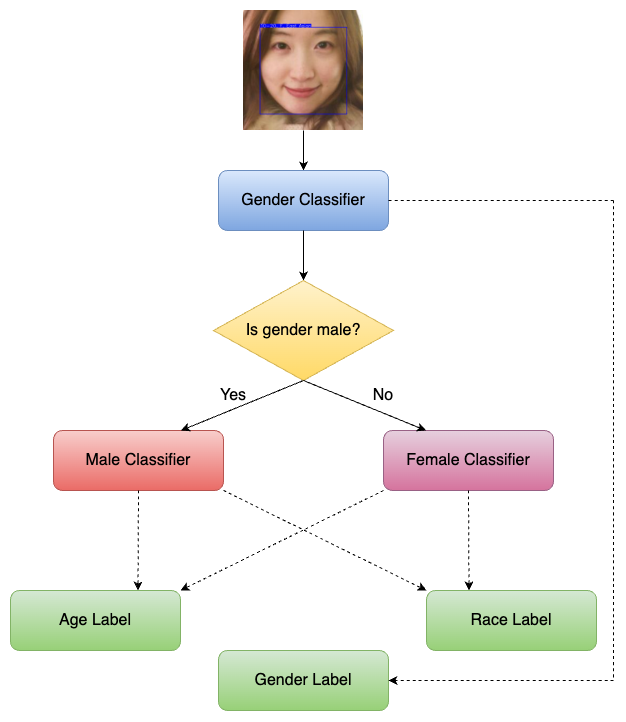
\includegraphics[width=1.0\linewidth]{imgs/fusion}
	\caption{Fusion Model Architecture}
	\label{fig:fusion}
	\end{figure}
	
	

	
	\begin{figure*}[h]
		\centering
		\subcaptionbox{}[.45\linewidth][c]{%
			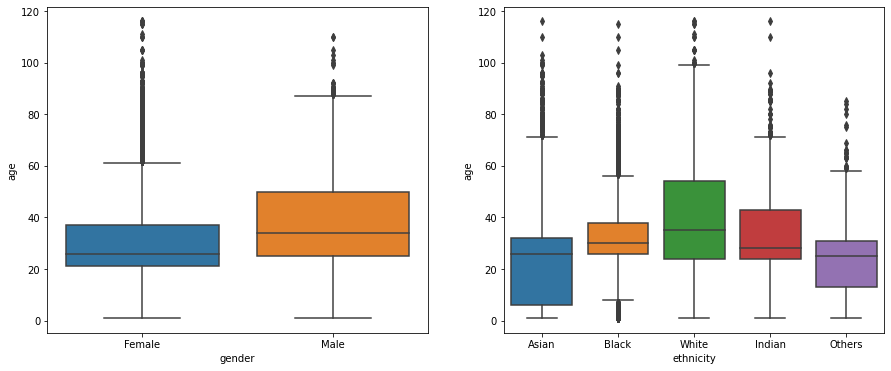
\includegraphics[width=\linewidth]{imgs/UTKface-data-ana1.png}}\quad
		\subcaptionbox{}[.45\linewidth][c]{%
			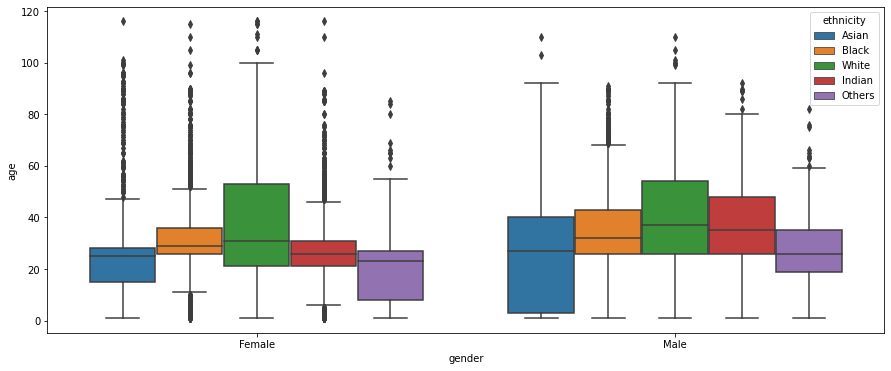
\includegraphics[width=\linewidth]{imgs/UTKface-data-ana2.png}}\quad
		\caption{UTKface data distribution}
		\label{fig:utkfacedist}
	\end{figure*}
	\section{Experiment}
	
	To solve the gender-age-race classification task, we first performed the gender-age prediction sub-task and then added the race prediction sub-task to enable the model to complete the ternary classification task. The popular IMDb-WIKI dataset was used for the gender-age prediction sub-task, and the UTKface and FairFace dataset was used for the additional race prediction sub-task, as there are no race labels in the IMDb-WIKI dataset. The sizes of different datasets vary, and there were multiple choices of pre-trained models, which guided us to determine which dataset-model combination to use. Hence we also studied the relationship between dataset size and model architecture by trying different backbones on IMDb-WIKI, and selected the top-performing network for use. As for the additional race prediction sub-task, we compared the performances of our pre-trained models including Xception and ResNet on UTKface and FairFace respectively to determine a better model and a more appropriate dataset for use. 
	
	
	With the obtained comparative results, we then selected FairFace as the target dataset and ResNet as the pre-trained model to perform our age-gender-race ternary classification task. In order to optimize the original model architecture and effectively harness the gender-specific information, we implemented a gender-specific fusion model with a two-stage architecture, and compared its performance over the original model.
	
	
	\subsection{Setup} \label{setup}
	
	\paragraph{Datasets.} As for the gender-age prediction sub-task, we used the IMDb-WIKI\cite{Rothe-IJCV-2018, Rothe-ICCVW-2015} with 460,723 images from IMDb and 62,328 images from Wikipedia, which have labeled ages and genders.
	
	\begin{figure}[H]
		\centering
		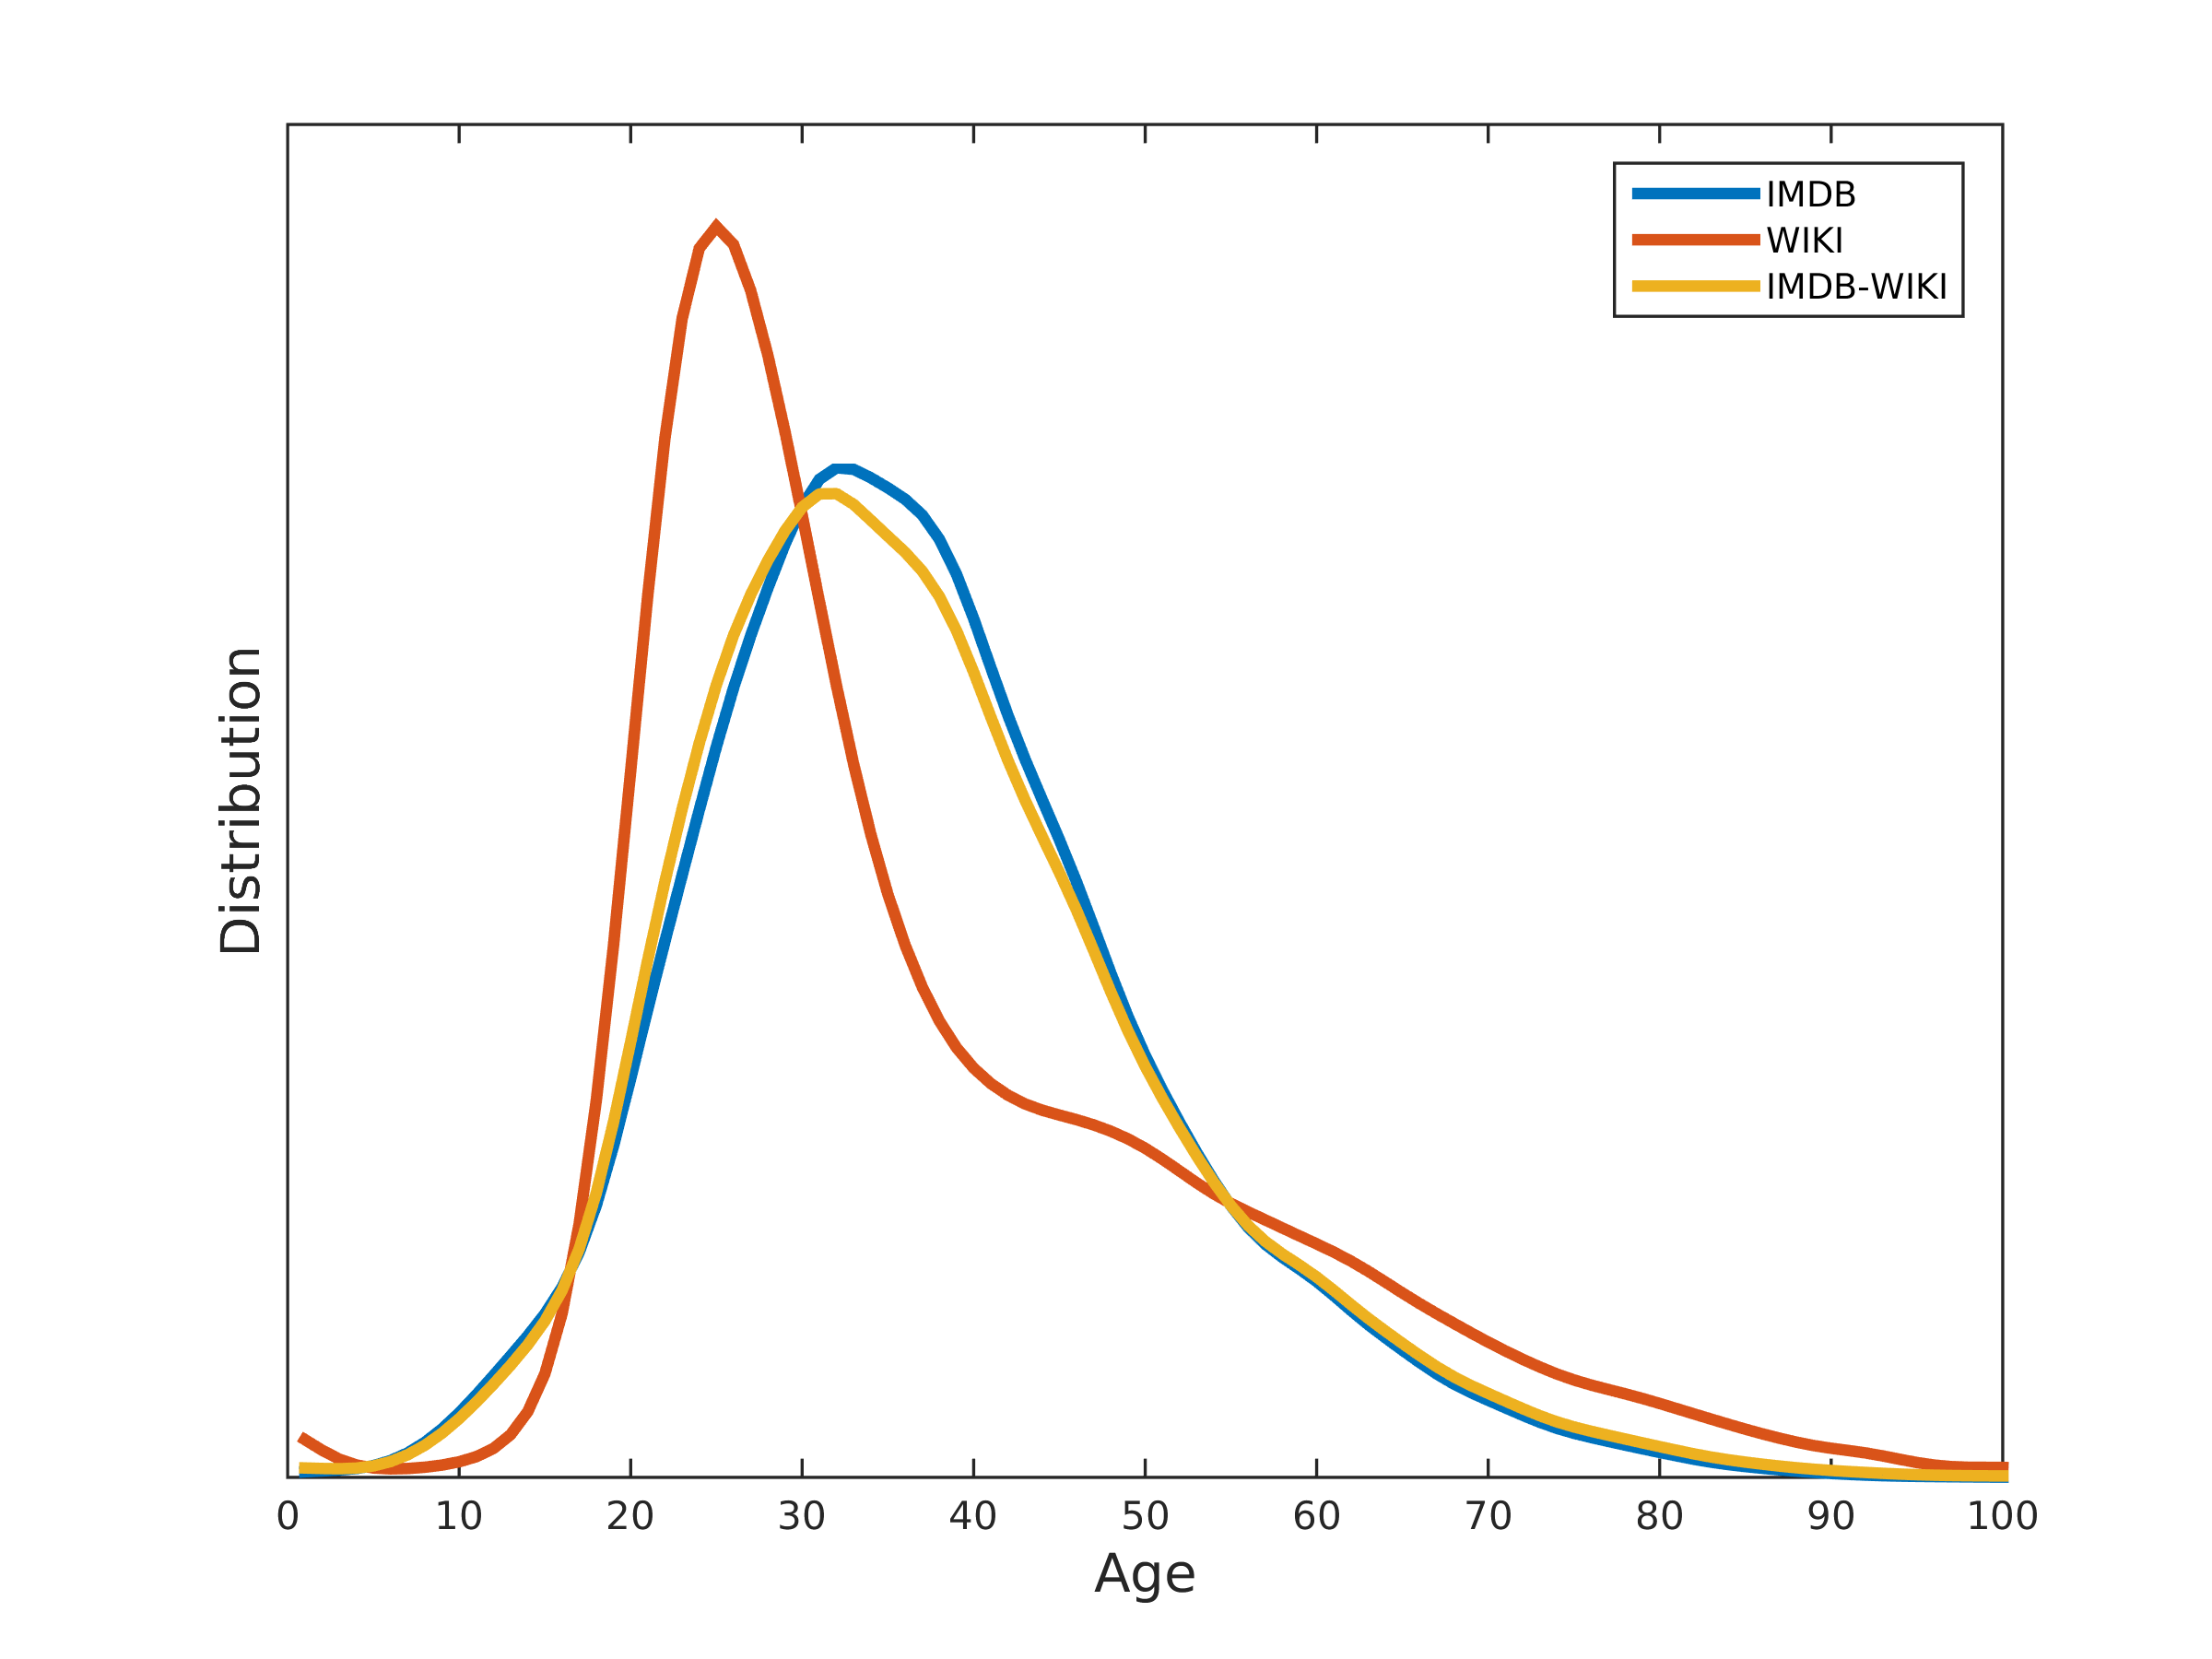
\includegraphics[width=0.7\linewidth]{imgs/screenshot001}
		\caption{Age distribution of IMDb-WIKI}
		\label{fig:screenshot001}
	\end{figure}
	
	As for the race prediction subtask, we evaluated our models on the UTKface\cite{zhifei2017cvpr} dataset and FairFace\cite{karkkainenfairface} dataset. The UTKface dataset contains 23706 images, with 2 genders: male and female, 117 classes of ages: 0 to 116, and 5 classes of races: White, Black, Asian, Indian, and Others. The models used 13275 examples for training, 3319 samples for evaluation, and the rest for testing. The race distribution and gender-specified age distributions are displayed in Figure \ref{fig:utkfacedist}. 
	
	The FairFace contains 108k faces with 2 genders, 9 classes of ages, and 7 classes of races. It has two sets: train and test. We utilized the training set for fine-tuning and the testing set for metrics. The race distribution of FairFace is more balanced compared to that of other datasets, as shown in Figure \ref{fig:screenshot002}.
	
	The pre-trained models were trained on ImageNet\cite{ILSVRC15} on the original validation labels. The last layer was dropped as the models were used for a different down-streaming task.
	
	\begin{figure}[H]
		\centering
		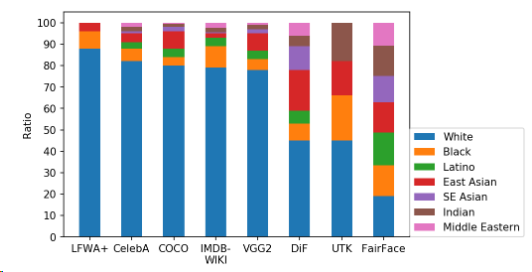
\includegraphics[width=1\linewidth]{imgs/screenshot002}
		\caption{Racial compositions in face datasets}
		\label{fig:screenshot002}
	\end{figure}
	
	\paragraph{Pretraining \& Fine-tuning.} To train our model, we utilized the pre-trained architectures and parameters. The pre-trained models were downloaded from Keras. In this assignment, we tried Xception, VGG19, ResNet152V2, InceptionResNetV2, MobileNetV2, and DenseNet201.
	
	We used adam optimizer with a learning rate $ 2e-4 $ to train on image size 224. For each model, we set the batch size to 32 and the maximum epoch number to 30 with early stopping to prevent over-fitting. We added additional classifier heads to the last layer of the network.
	
	\paragraph{Metrics.} The performance of our fine-tuned models was evaluated on the test set of UTKface. We calculated both loss and accuracy to evaluate the model performance.
	
	\subsection{Experiments on the backbone}\label{sec:backbone}
	To select the top-performing backbones, we evaluated the pre-trained models including Xception, VGG19, ResNet152V2, InceptionResNetV2, MobileNetV2, and DenseNet on the IMDb and Wiki dataset. The result is shown in table \ref{wiki-imdb-table}.
	
	\begin{table*}[t]
		\centering
		\begin{tabular}{ccccccc}
			\hline
			\multicolumn{2}{c}{}                                                                & loss  & val gender acc & test gender acc & val age acc & test age acc \\ \hline
			\multicolumn{1}{c|}{\multirow{2}{*}{Xception}}          & \multicolumn{1}{c|}{IMDb} & 3.442 & 0.912          & 0.821           & 0.102       & 0.036        \\ \cline{2-2}
			\multicolumn{1}{c|}{}                                   & \multicolumn{1}{c|}{Wiki} & 3.403 & 0.971          & 0.815           & 0.082       & 0.059        \\ \cline{1-2}
			\multicolumn{1}{c|}{\multirow{2}{*}{VGG19}}             & \multicolumn{1}{c|}{IMDb} & 3.749 & 0.899          & 0.721           & 0.063       & 0.035        \\ \cline{2-2}
			\multicolumn{1}{c|}{}                                   & \multicolumn{1}{c|}{Wiki} & 3.887 & 0.924          & 0.629           & 0.052       & 0.033        \\ \cline{1-2}
			\multicolumn{1}{c|}{\multirow{2}{*}{ResNet152V2}}       & \multicolumn{1}{c|}{IMDb} & 3.924 & 0.893          & 0.767           & 0.052       & 0.036        \\ \cline{2-2}
			\multicolumn{1}{c|}{}                                   & \multicolumn{1}{c|}{Wiki} & 3.397 & 0.967          & 0.731           & 0.066       & 0.020        \\ \cline{1-2}
			\multicolumn{1}{c|}{\multirow{2}{*}{InceptionResNetV2}} & \multicolumn{1}{c|}{IMDb} & 3.464 & 0.913          & 0.794           & 0.119       & 0.033        \\ \cline{2-2}
			\multicolumn{1}{c|}{}                                   & \multicolumn{1}{c|}{Wiki} & 3.400 & 0.975          & 0.752           & 0.073       & 0.047        \\ \cline{1-2}
			\multicolumn{1}{c|}{\multirow{2}{*}{MobileNetV2}}       & \multicolumn{1}{c|}{IMDb} & 3.487 & 0.915          & 0.813           & 0.086       & 0.036        \\ \cline{2-2}
			\multicolumn{1}{c|}{}                                   & \multicolumn{1}{c|}{Wiki} & 3.352 & 0.975          & 0.812           & 0.063       & 0.037        \\ \cline{1-2}
			\multicolumn{1}{c|}{\multirow{2}{*}{DenseNet}}          & \multicolumn{1}{c|}{IMDb} & 3.491 & 0.915          & 0.826           & 0.091       & 0.037        \\ \cline{2-2}
			\multicolumn{1}{c|}{}                                   & \multicolumn{1}{c|}{Wiki} & 3.324 & 0.972          & 0.767           & 0.066       & 0.040        \\ \cline{1-2}
		\end{tabular}
		\caption{This table displays the results of the pre-trained backbones fine-tuned on different datasetss. The loss is tested on the validation set of the IMDb and Wiki dataset. The gender and age accuracies are validated on the validation set of the IMDb and Wiki dataset (val gender\&age acc) and tested on the UTKface dataset dropping the race label (test gender\&age acc).}
		\label{wiki-imdb-table}
	\end{table*}

	We reported the loss on validation set, gender accuracy on validation set, test gender accuracy on UTKface (race label dropped), age accuracy on validation set, age accuracy on UTKface over the models trained with different backbones and datasets. The accuracy on validation set roughly represents the model performance. Considering the size of dataset and different distributions of data between the IMDb and Wiki's validation set, we added an additional evaluation step on UTKface (race label dropped) for a more intuitive comparison.
	
	Among all the models, in general, the Xception and DenseNet are the top-performing models, and the VGG19 has the worst performance. For the gender classification, the DenseNet outperforms all the rest and achieves 82.6\% accuracy on the testing set. For the age classification, the Xception outperforms all the rest and achieves 5.6\% on the testing set. Noted that Xception is a relatively simpler architecture, and hence it is not easy to over-fit. By comparison, ResNet is more complex, and hence it may tend to overfit in the datasets above. However, it is still possible to use techniques like dropouts to mitigate the overfitting problem.
	
	To estimate the overfitting of each model, we enumerated the number of epochs for each model in table \ref{table:epochs}. By implementing early stopping, the fewer the training epochs are, the easier this model tends to overfit.
	
	According to Table 2, ResNet stops the earliest among all models, and VGG19 is the last to converge. This demonstrates that the dataset might be too small for fine-tuning ResNet and it might be too big for VGG19.
	
	\begin{table}[H]
		\centering
		\begin{tabular}{|c|c|c|}
			\hline
			\multirow{2}{*}{Xception}          & IMDb & 13 \\ \cline{2-3} 
			& Wiki & 12 \\ \hline
			\multirow{2}{*}{VGG19}             & IMDb & 25 \\ \cline{2-3} 
			& Wiki & 30 \\ \hline
			\multirow{2}{*}{ResNet152V2}       & IMDb & 5  \\ \cline{2-3} 
			& Wiki & 12 \\ \hline
			\multirow{2}{*}{InceptionResNetV2} & IMDb & 13 \\ \cline{2-3} 
			& Wiki & 11 \\ \hline
			\multirow{2}{*}{MobileNetV2}       & IMDb & 20 \\ \cline{2-3} 
			& Wiki & 19 \\ \hline
			\multirow{2}{*}{DenseNet}          & IMDb & 12 \\ \cline{2-3} 
			& Wiki & 12 \\ \hline
		\end{tabular}
		\caption{Number of epochs}
		\label{table:epochs}
	\end{table}
	
	
	Noted that the age accuracies are relatively low, which are around 30\%-50\% for different backbones on the test set. One possible reason is that there are 101 age classes in the WIKI-IMDb dataset. When considering each age as a separate class, the age features for the neighboring ages are too similar so it is hard for model, even human, to predict the exact age class correctly. The cross-entropy is calculated with this label policy by one-hot strategy so that even though the model's prediction is close to the ground truth, it is still considered as a "wrong prediction". Hence, the label policy leads to the relatively poor outcomes. This guides us to use age group as the output label to reduce the number of output classes.
	
	\subsection{Experiments on the size of dataset}
	
	As we discussed in section \ref{setup}, the IMDb dataset is around ten times larger than Wiki dataset. Hence, we could study the effects of dataset size by comparing the performances between IMDb and Wiki.
	
	For the gender accuracy, all the models fine-tuned on IMDb achieved better results than those fine-tuned on Wiki. For the age accuracy, four out of the six models fine-tuned on Wiki achieved better results than those fine-tuned on IMDb. This indicates that it is not always the case that training on a larger dataset will lead to a better model performance. The distributions and quality of the data might also affect the effectiveness of training. We should not always select the largest dataset for use, instead, a more complete data analysis should be performed on the dataset and then make a decision.
	
	\paragraph{Stability.} The size of dataset may have an impact on the stability during training. A large dataset could make the model converge more stably most of the time. This helps prevent the model from oscillating around the convergence point to some extent.
	
	We take the val\_loss of Xception shown in figure \ref{fig:oscillation} as an example.
	
	\begin{figure}[H]
		\centering
		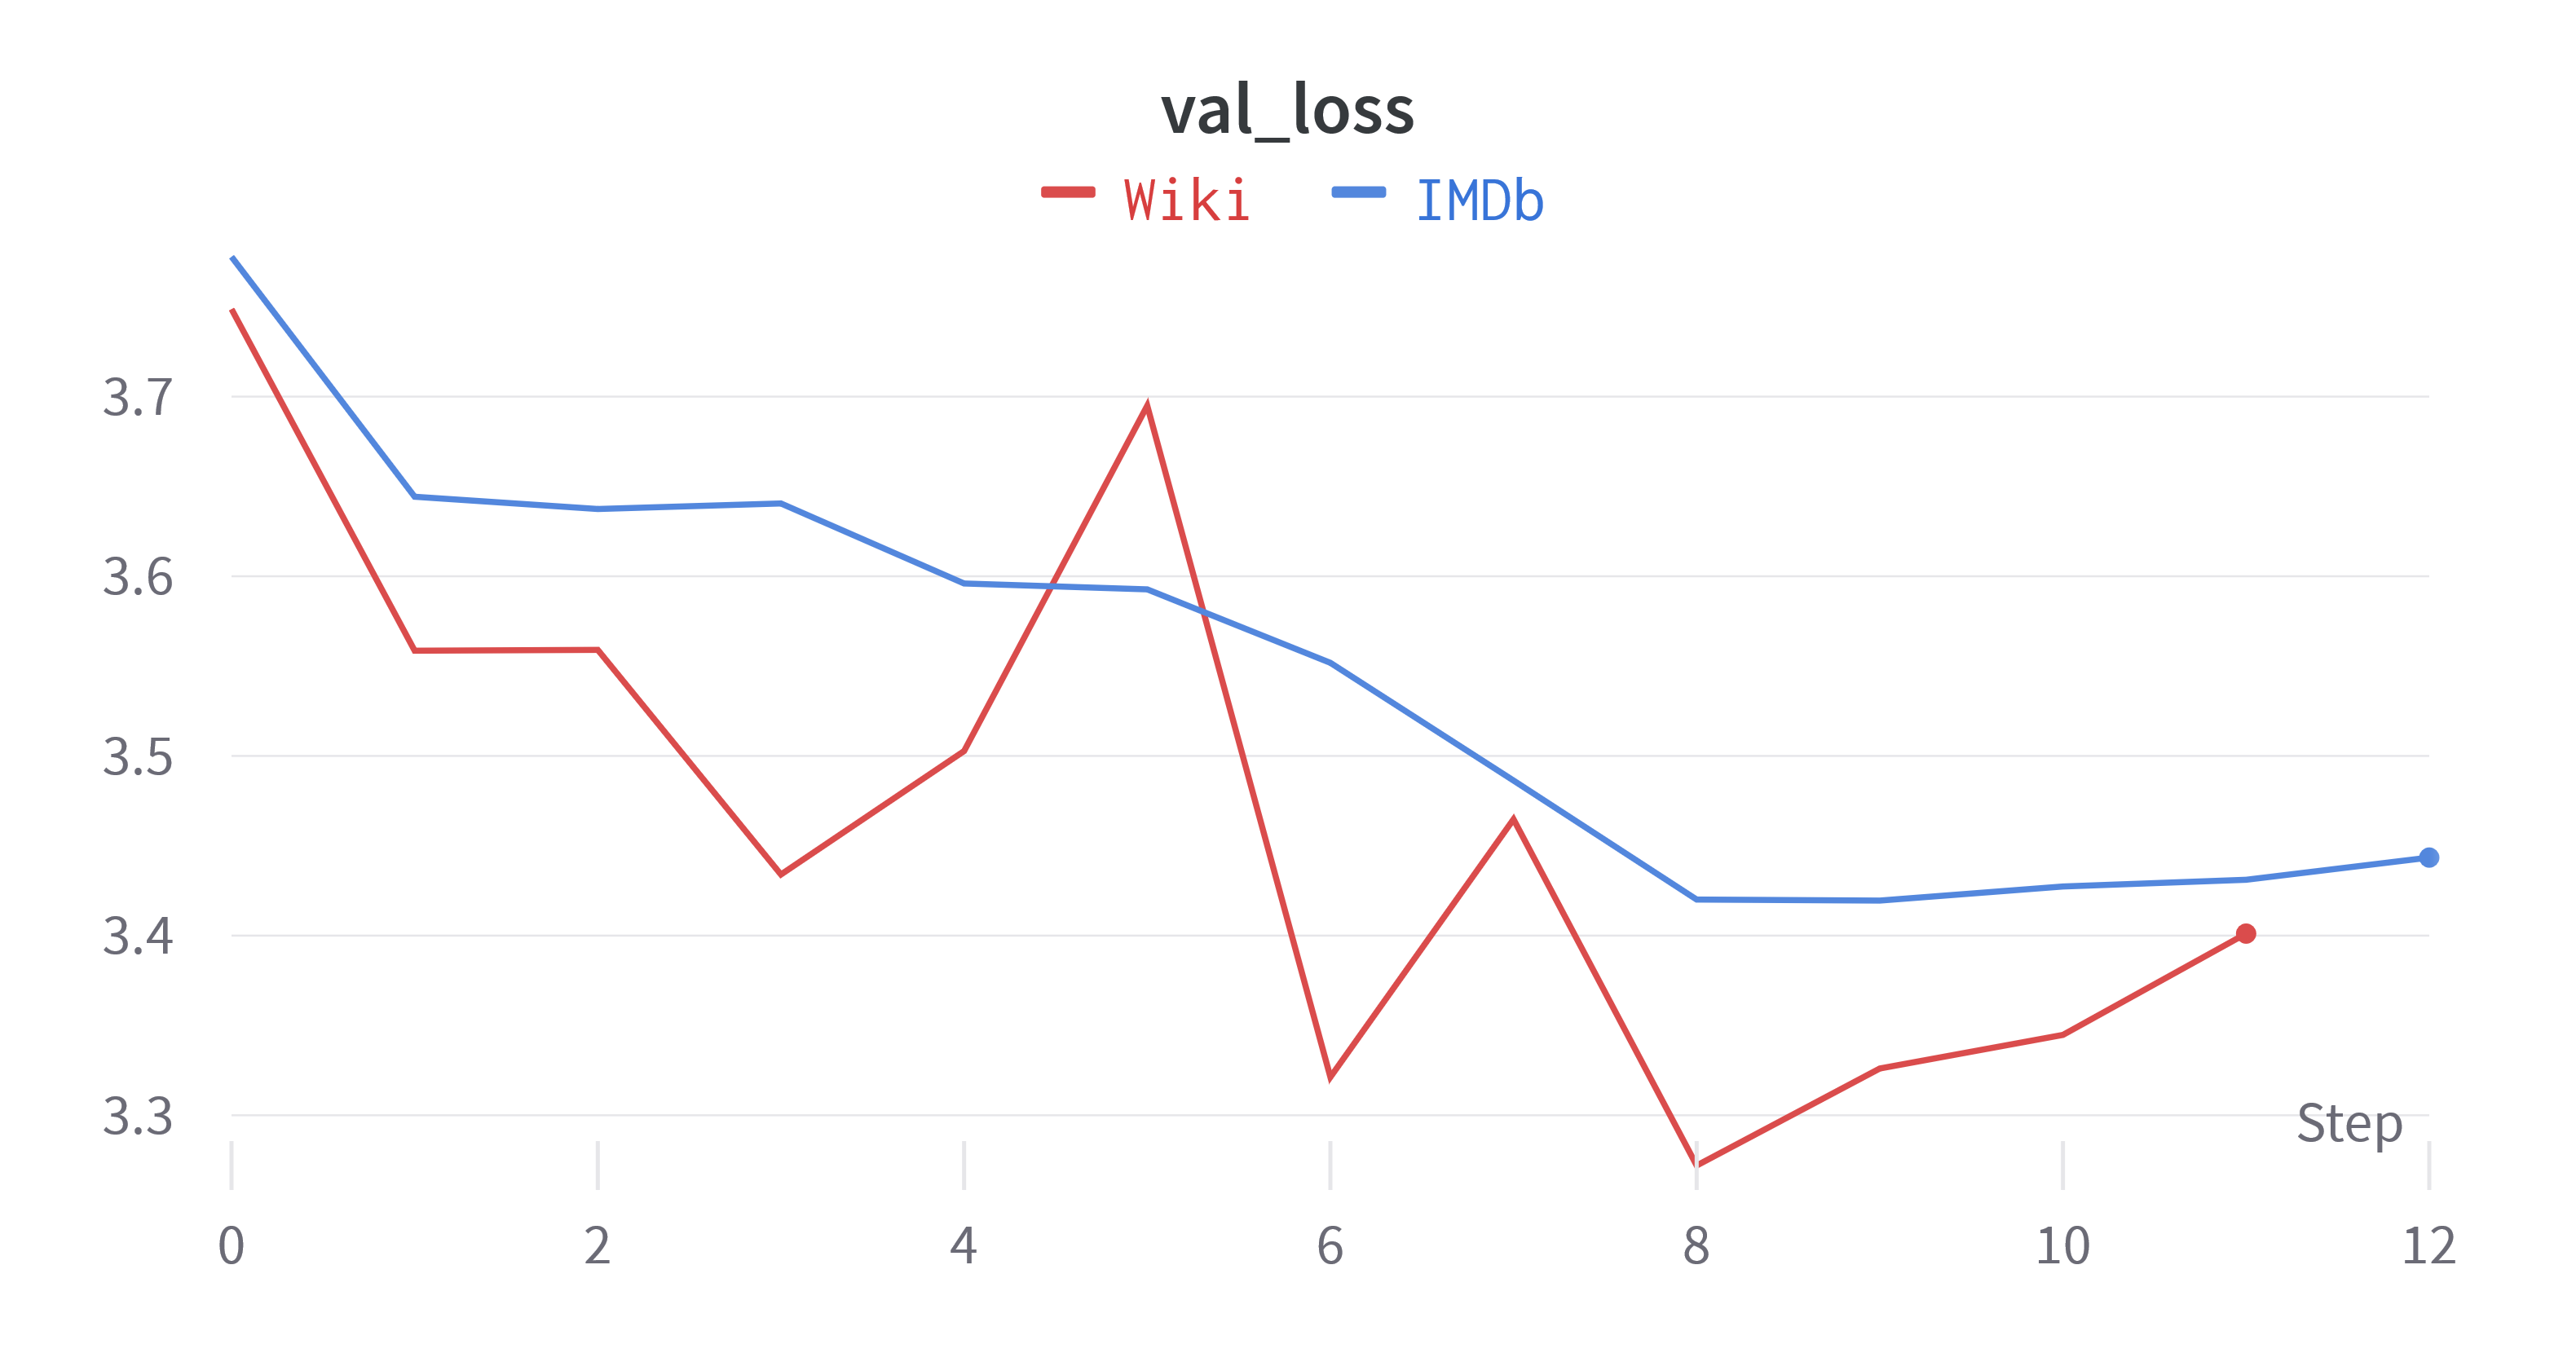
\includegraphics[width=0.7\linewidth]{imgs/oscillation}
		\caption{Stability of training}
		\label{fig:oscillation}
	\end{figure}
	
	Even though the final loss of model on Wiki is smaller, it oscillates heavily. This corresponds to our previous analysis.
	
	\begin{figure*}[t]
		\centering
		\subcaptionbox{}[.3\linewidth][c]{%
			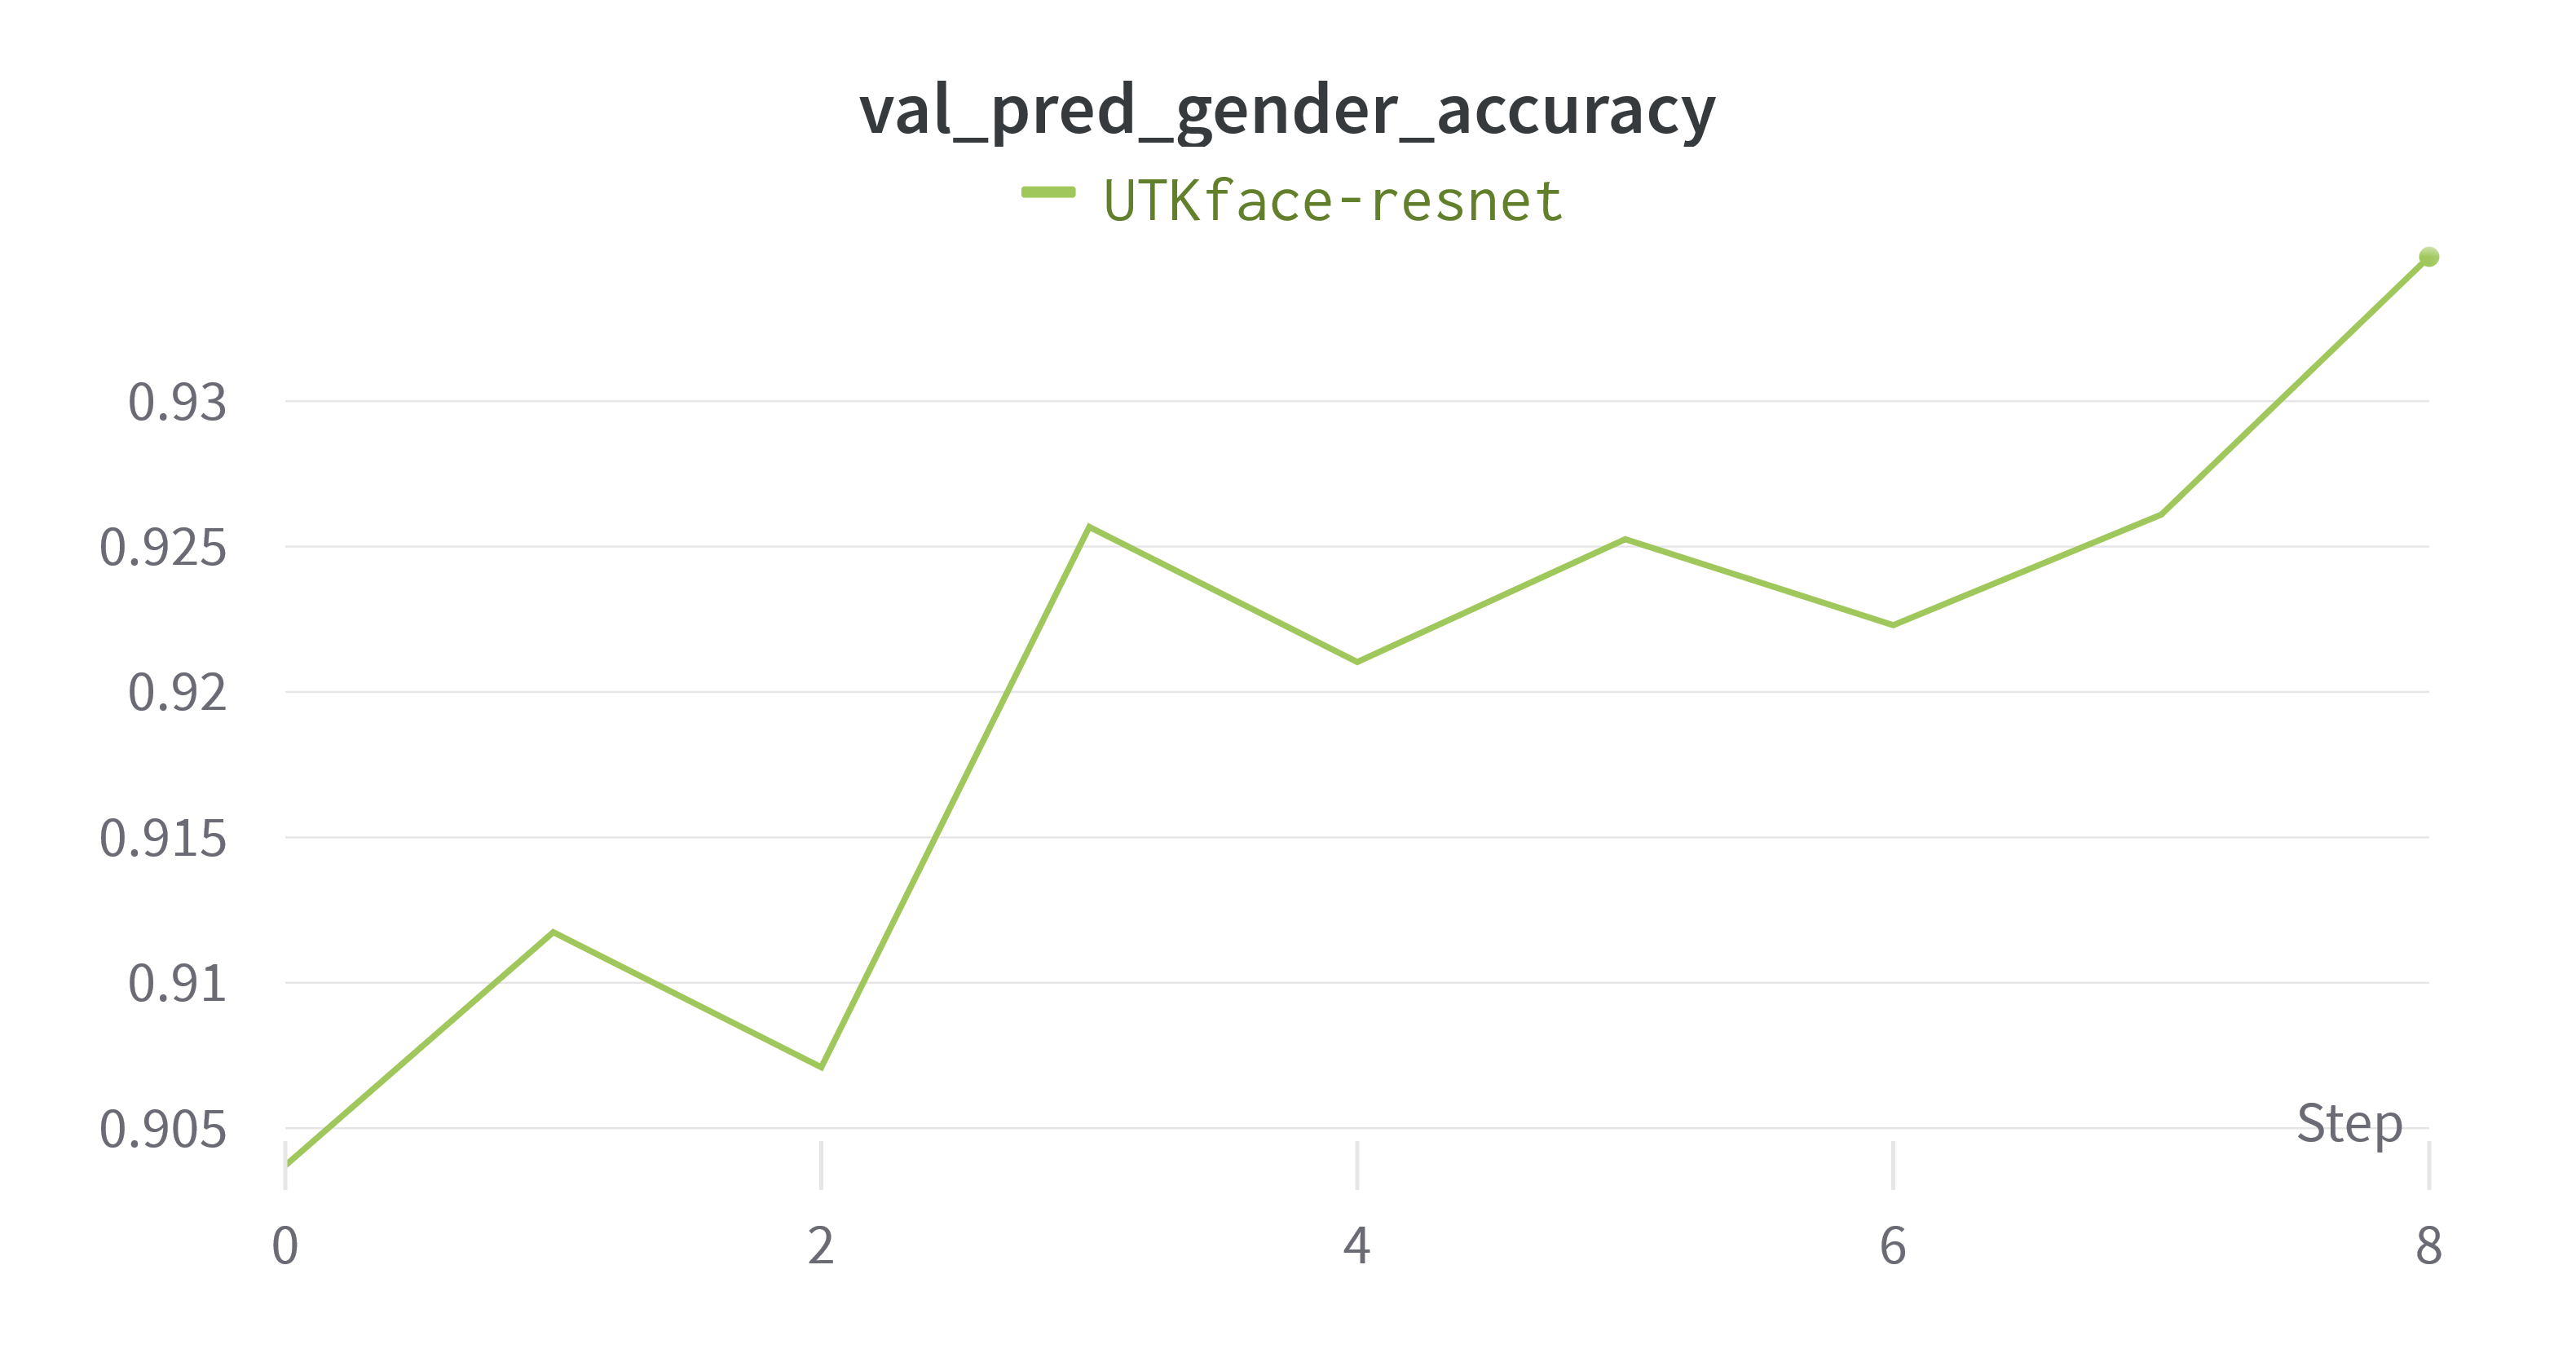
\includegraphics[width=\linewidth]{imgs/UTKface-resnet-gender.png}}\quad
		\subcaptionbox{}[.3\linewidth][c]{%
			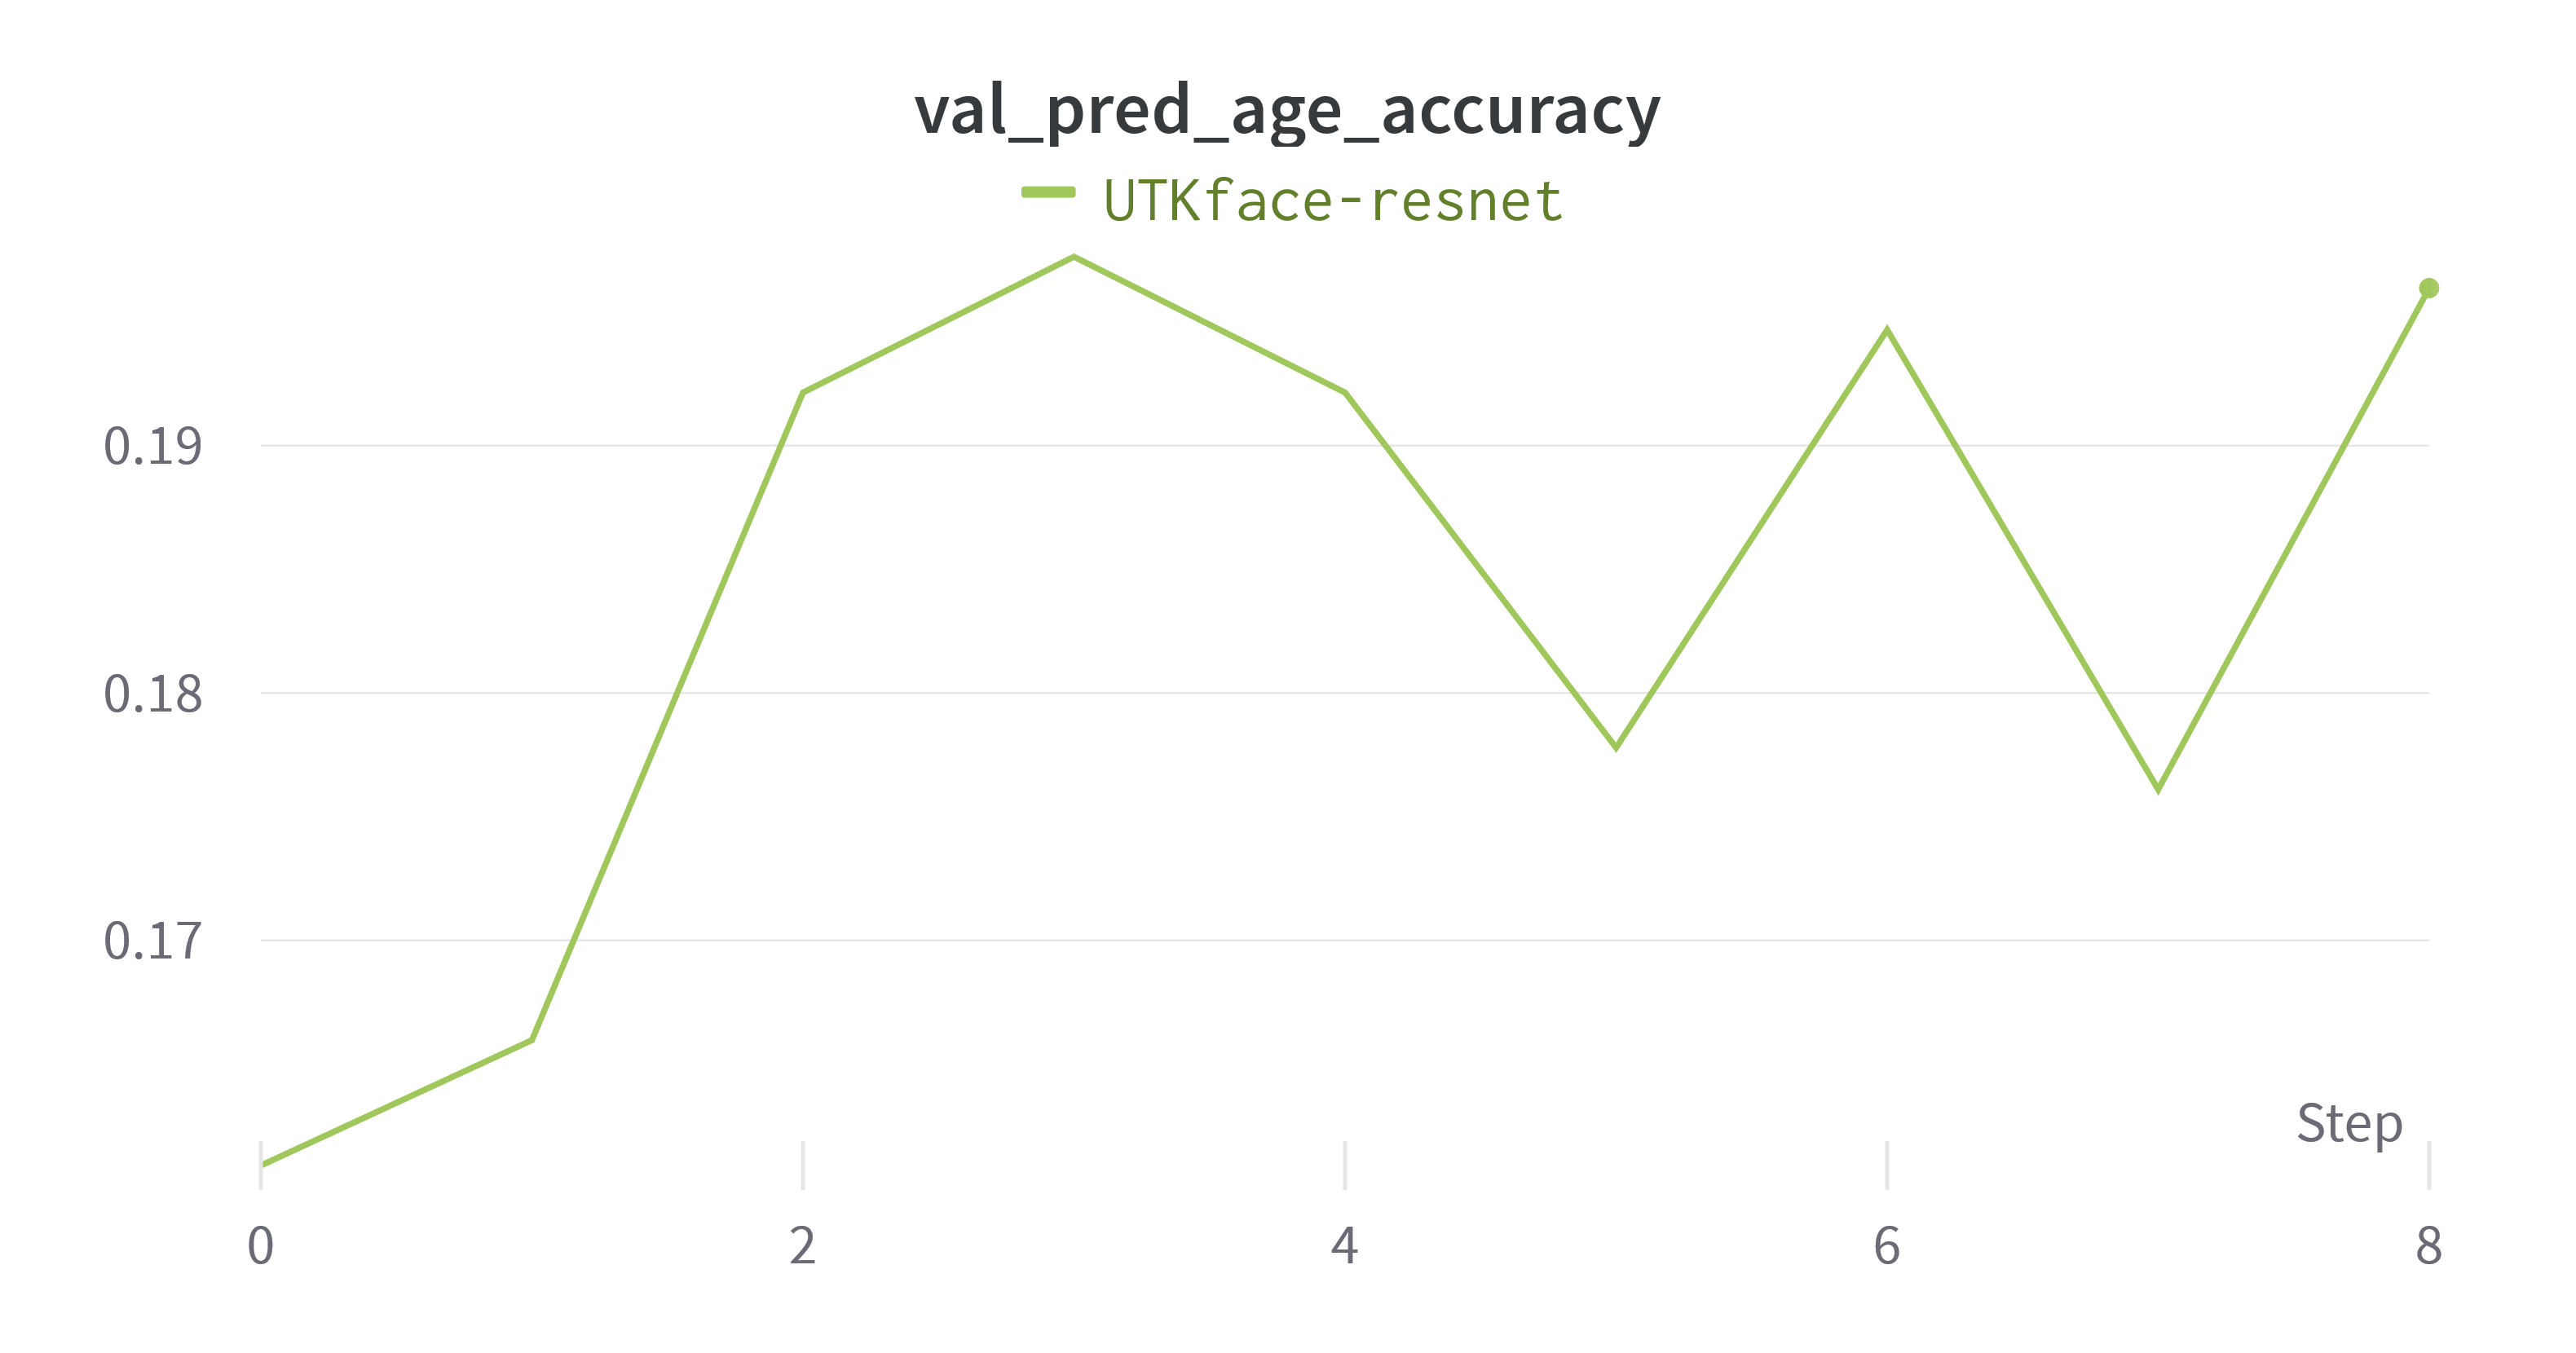
\includegraphics[width=\linewidth]{imgs/UTKface-resnet-age.png}}\quad
		\subcaptionbox{}[.3\linewidth][c]{%
			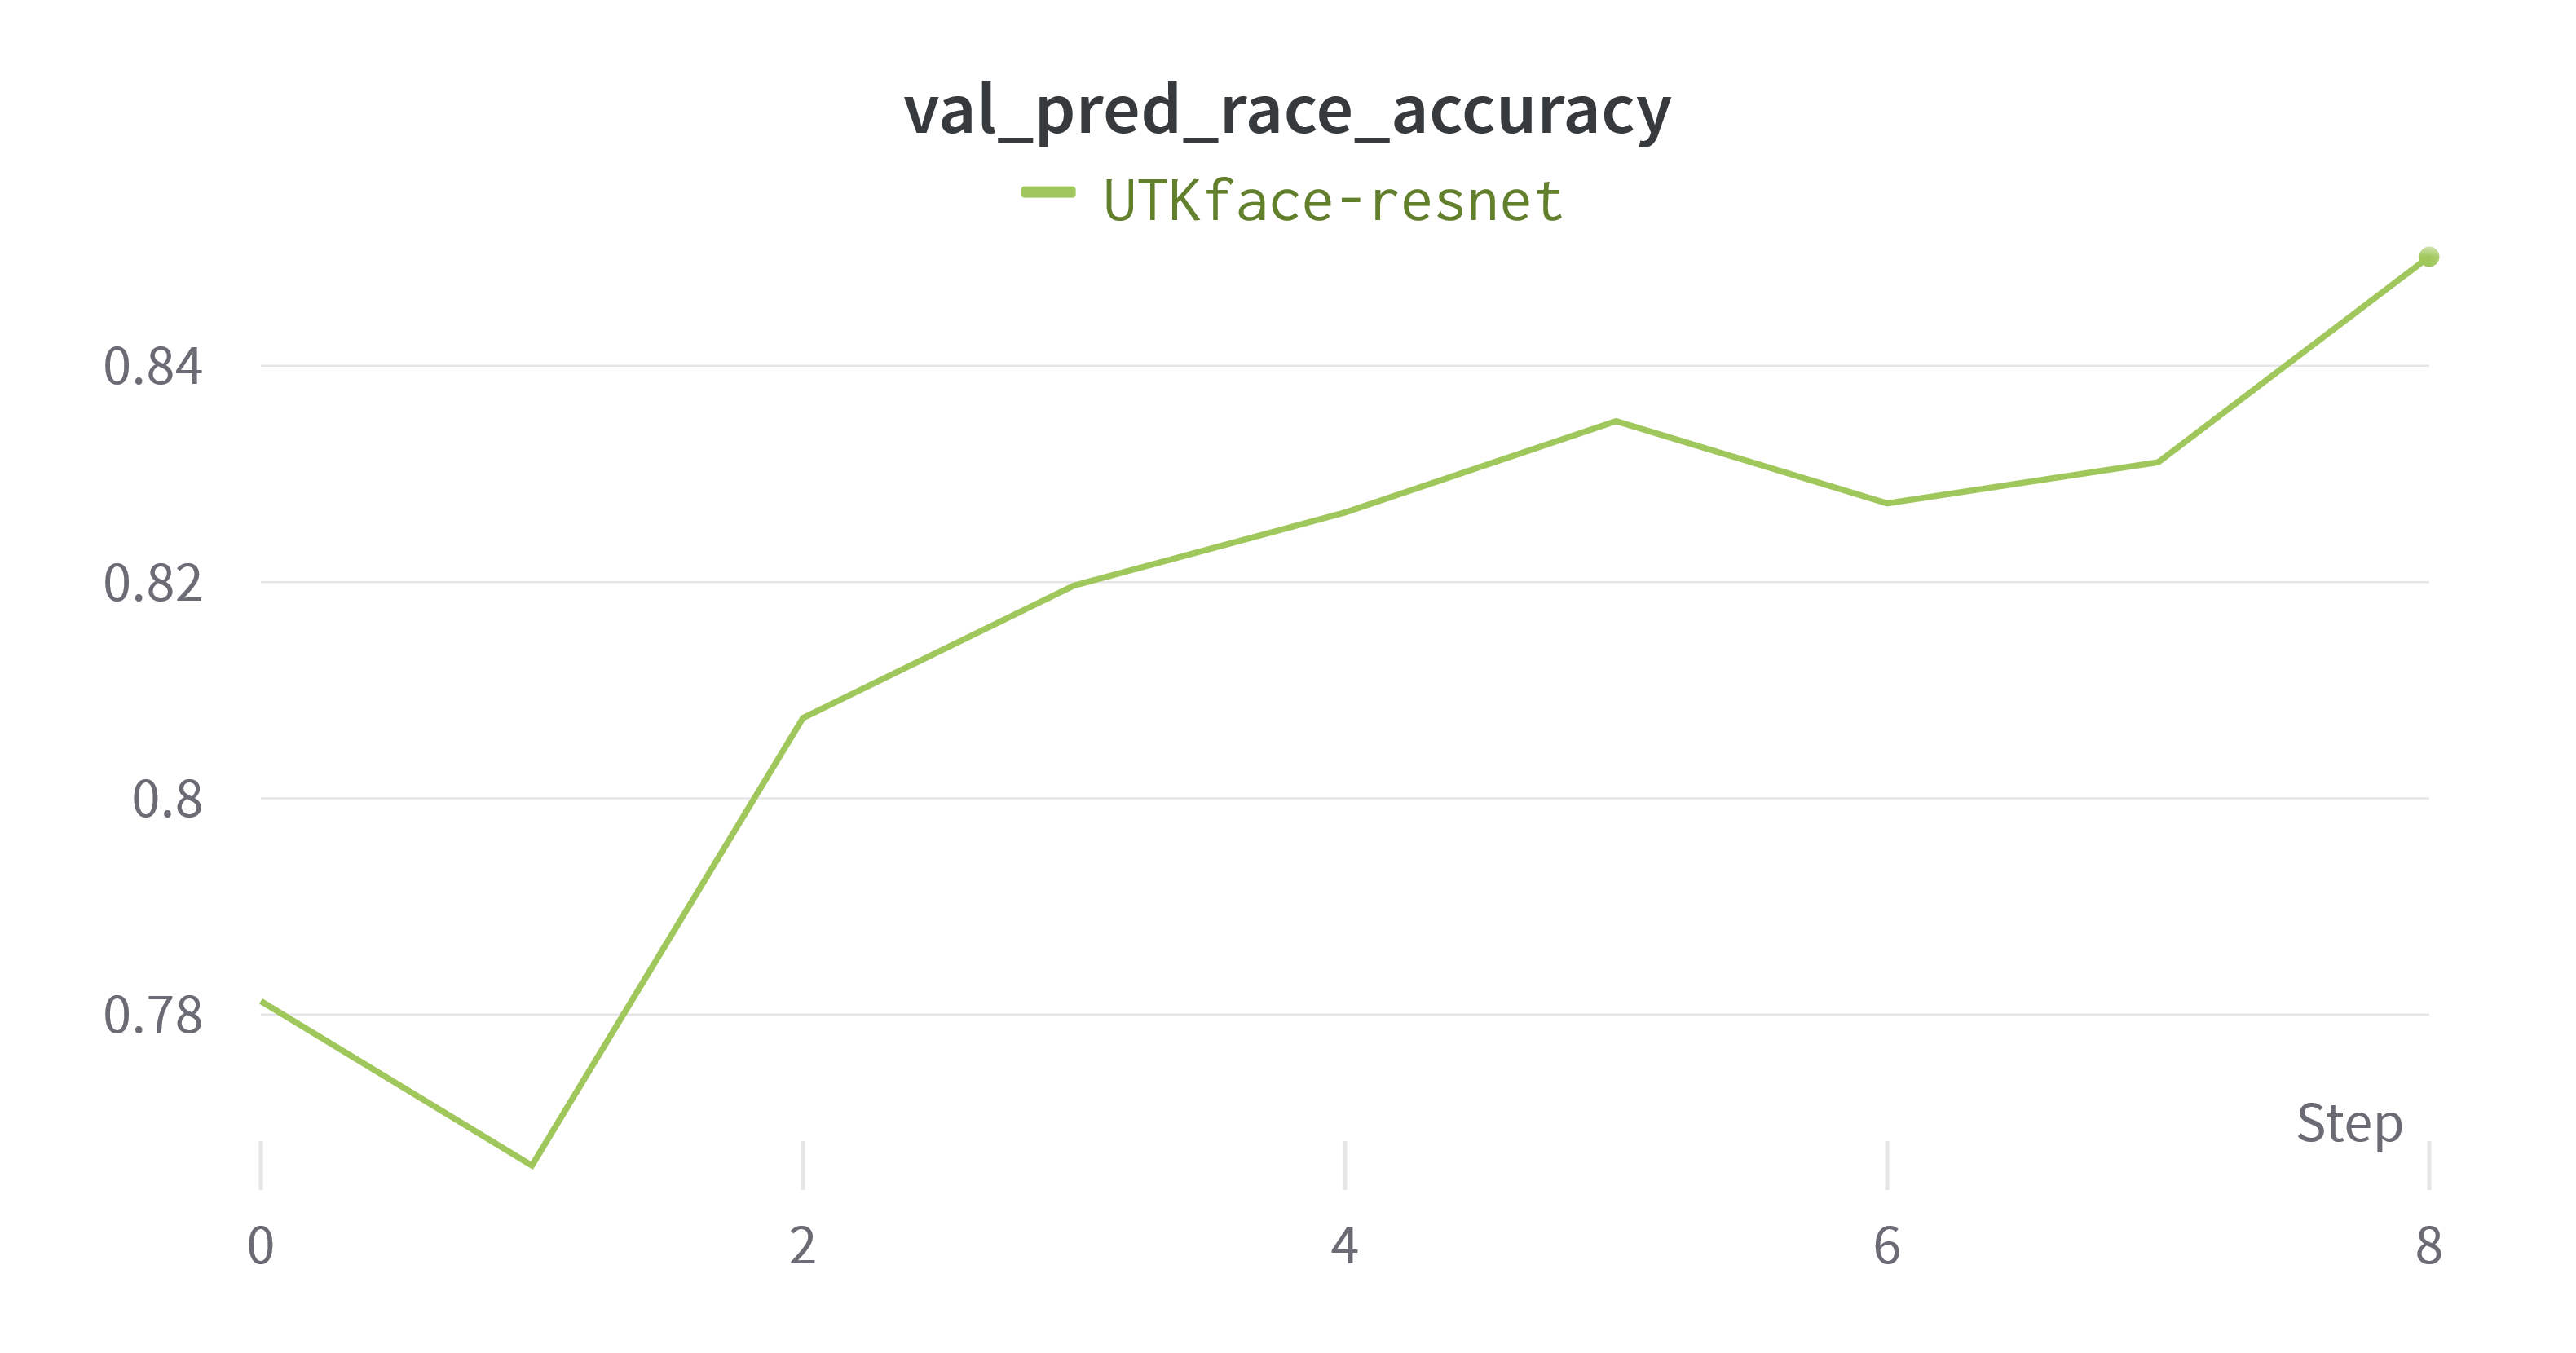
\includegraphics[width=\linewidth]{imgs/UTKface-resnet-race.png}}
		
		\bigskip
		
		\subcaptionbox{}[.3\linewidth][c]{%
			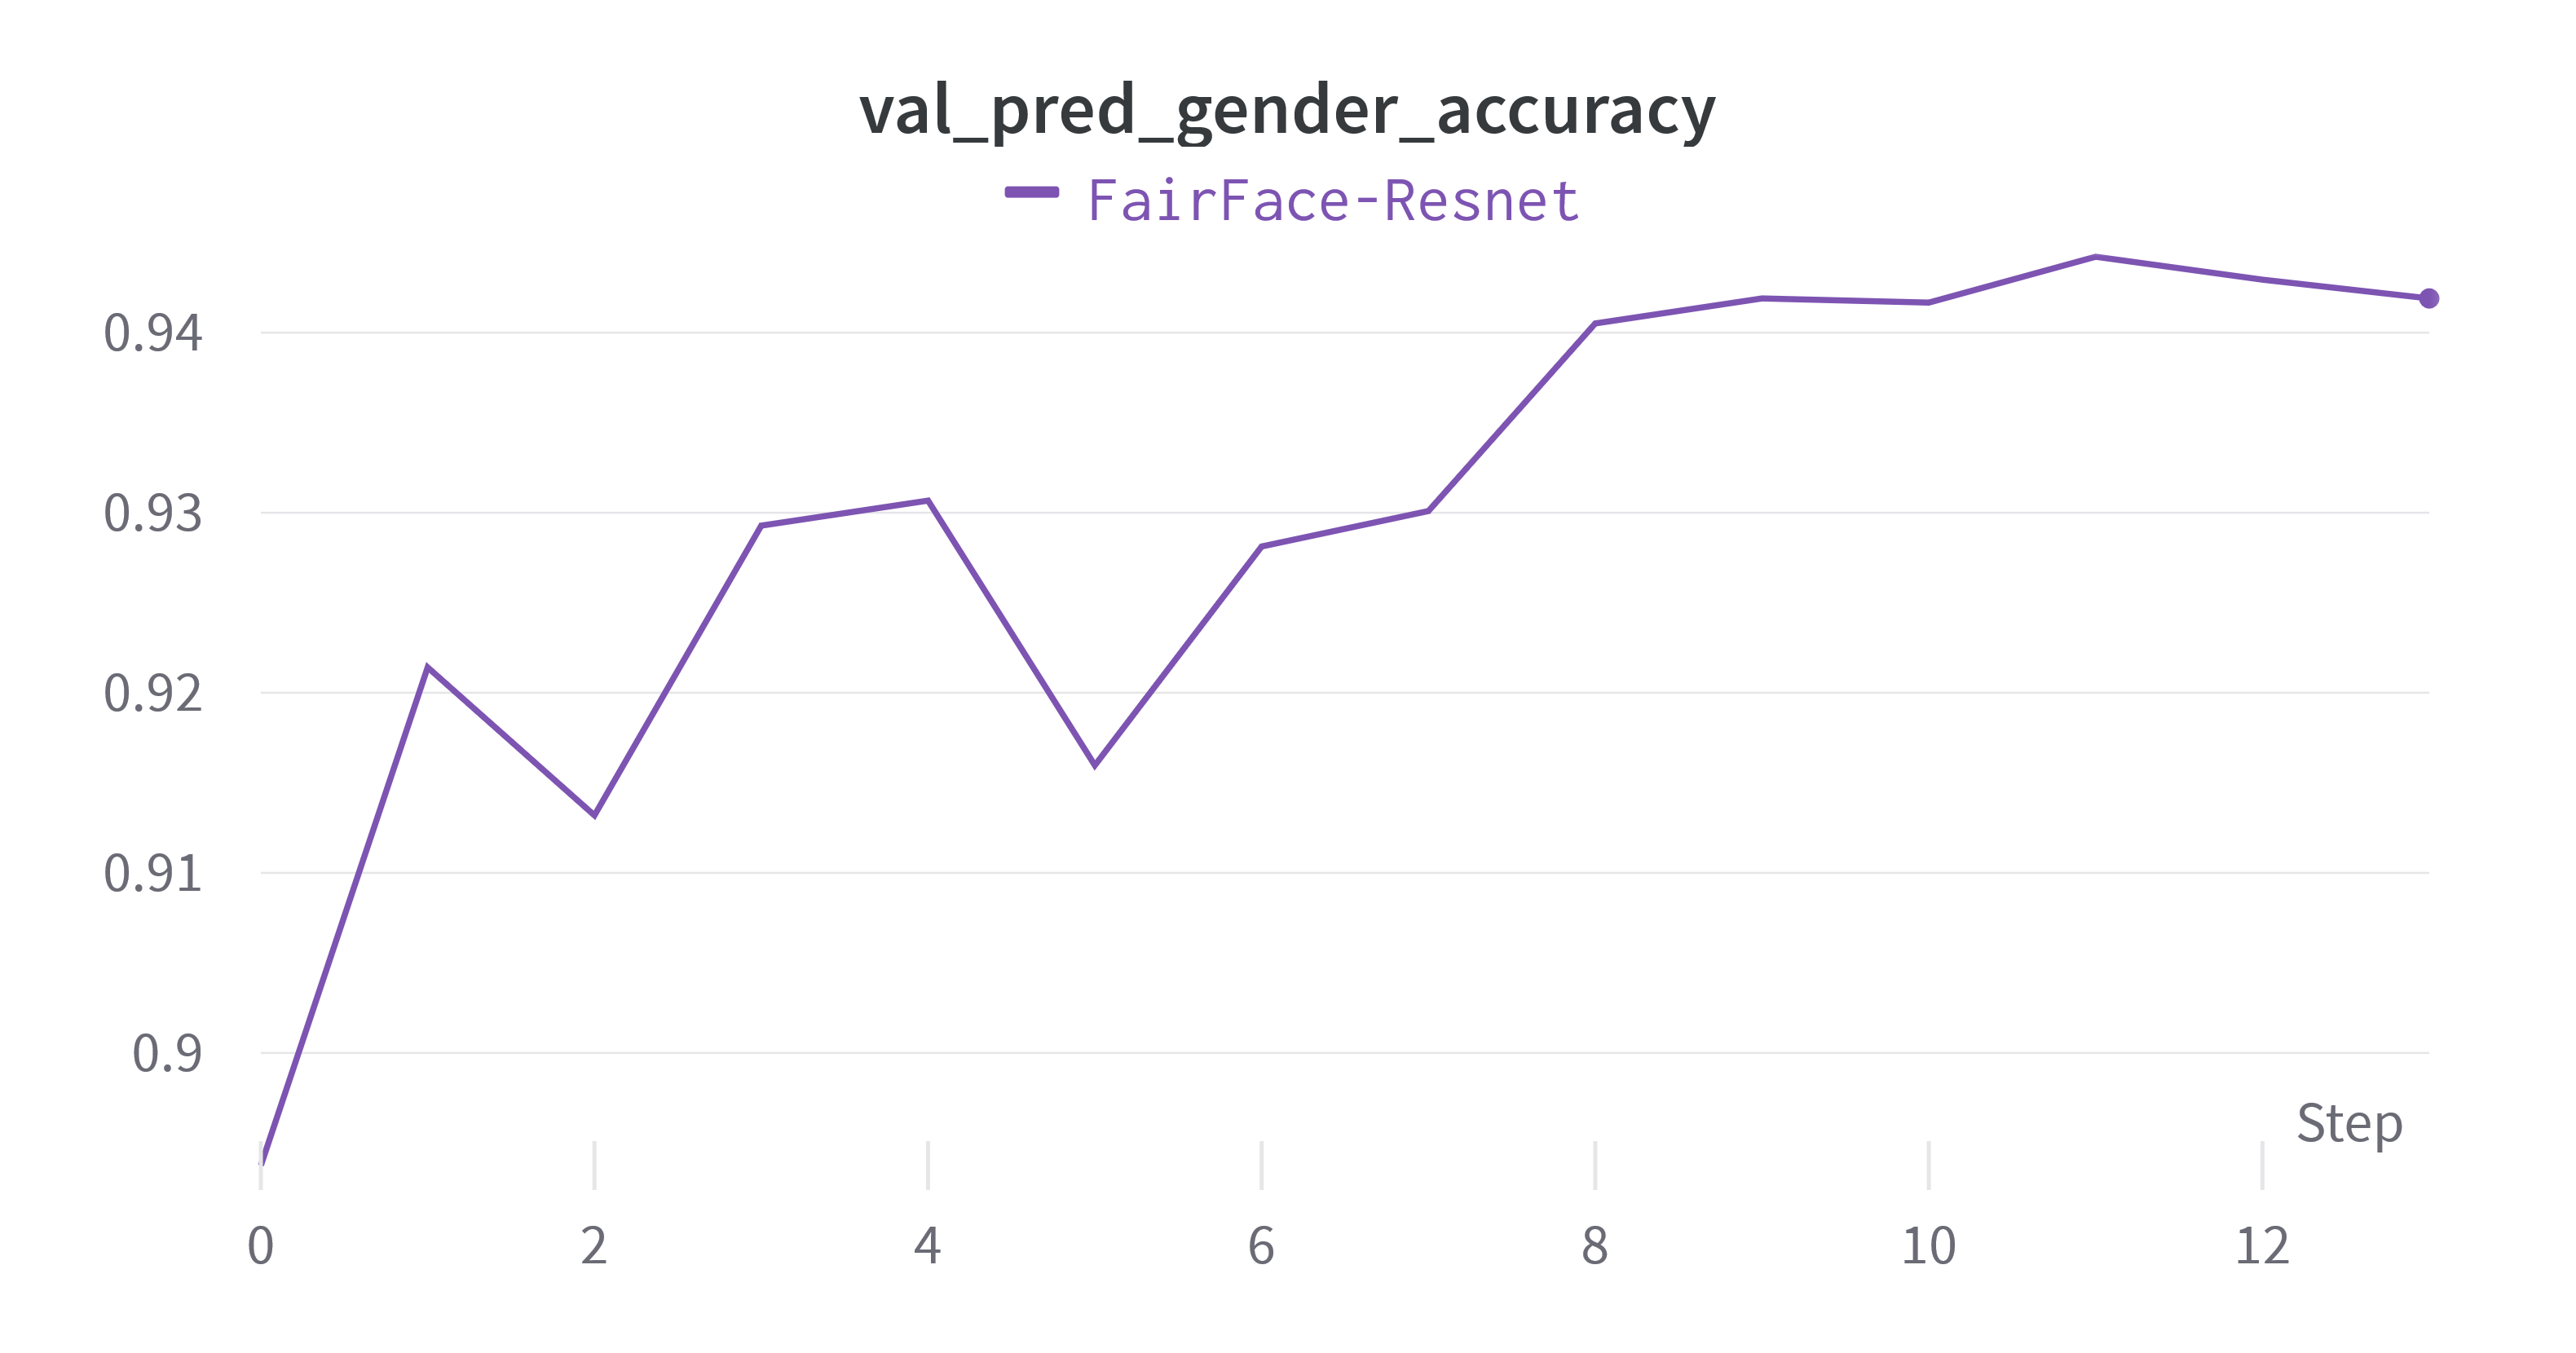
\includegraphics[width=\linewidth]{imgs/FairFace-resnet-gender.png}}\quad
		\subcaptionbox{}[.3\linewidth][c]{%
			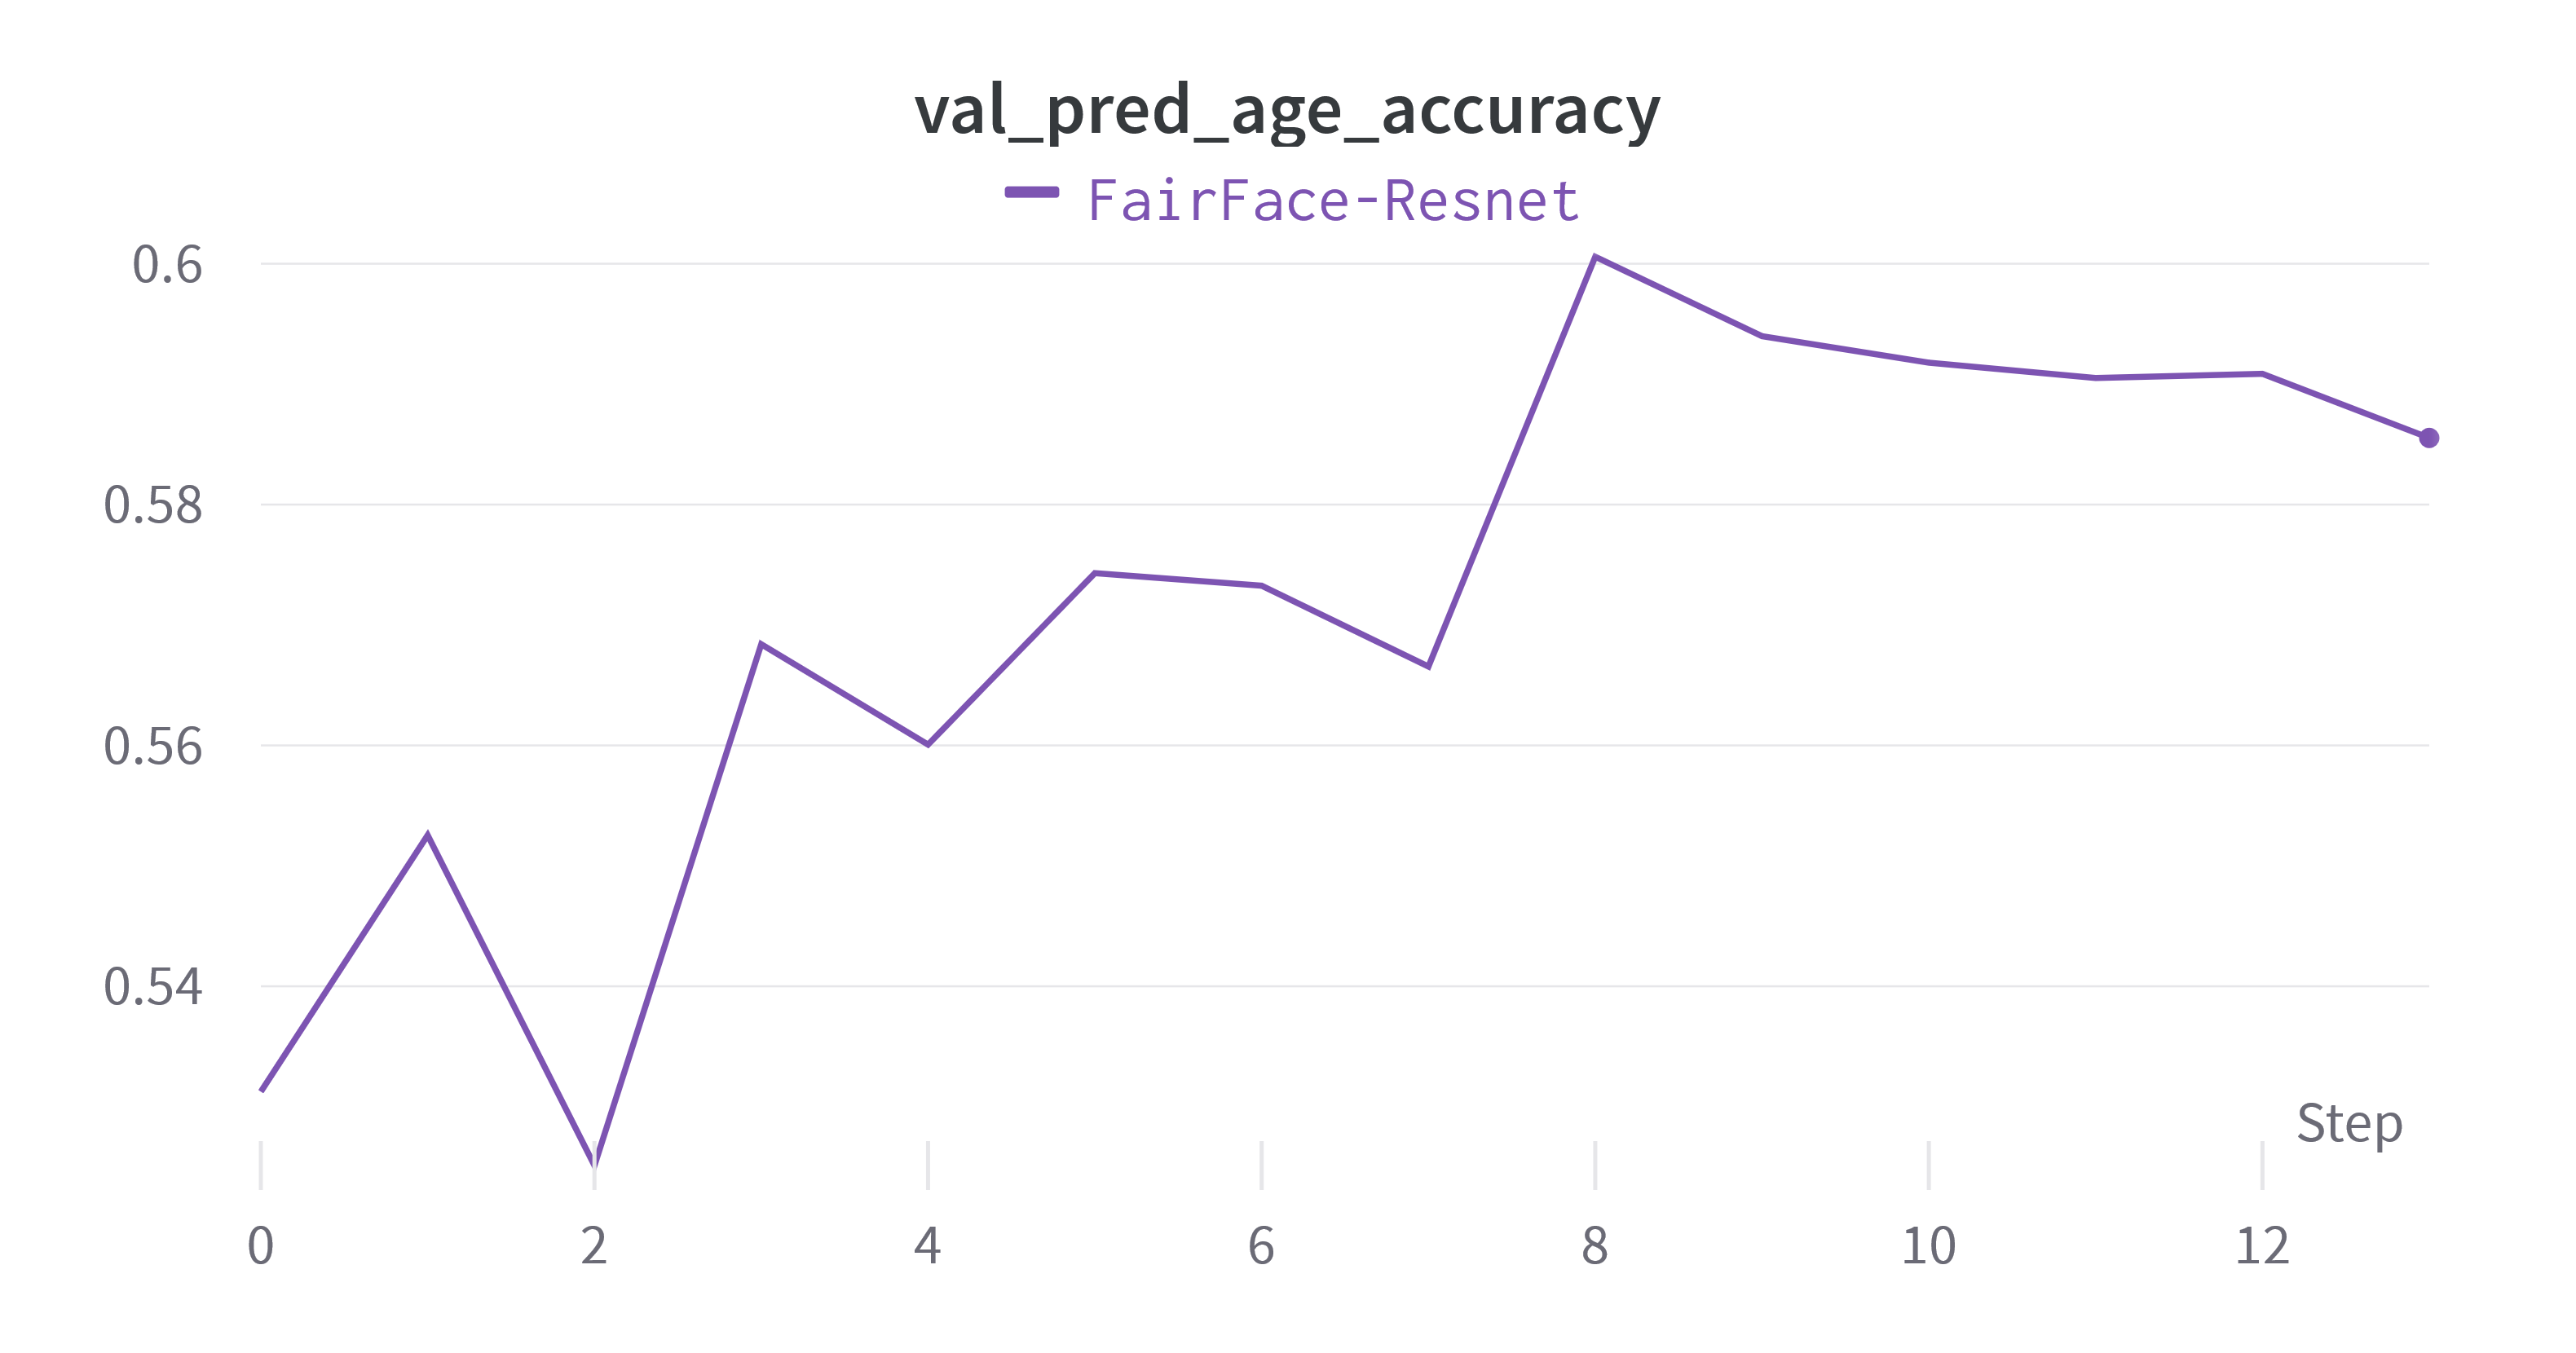
\includegraphics[width=\linewidth]{imgs/FairFace-resnet-age.png}}\quad
		\subcaptionbox{}[.3\linewidth][c]{%
			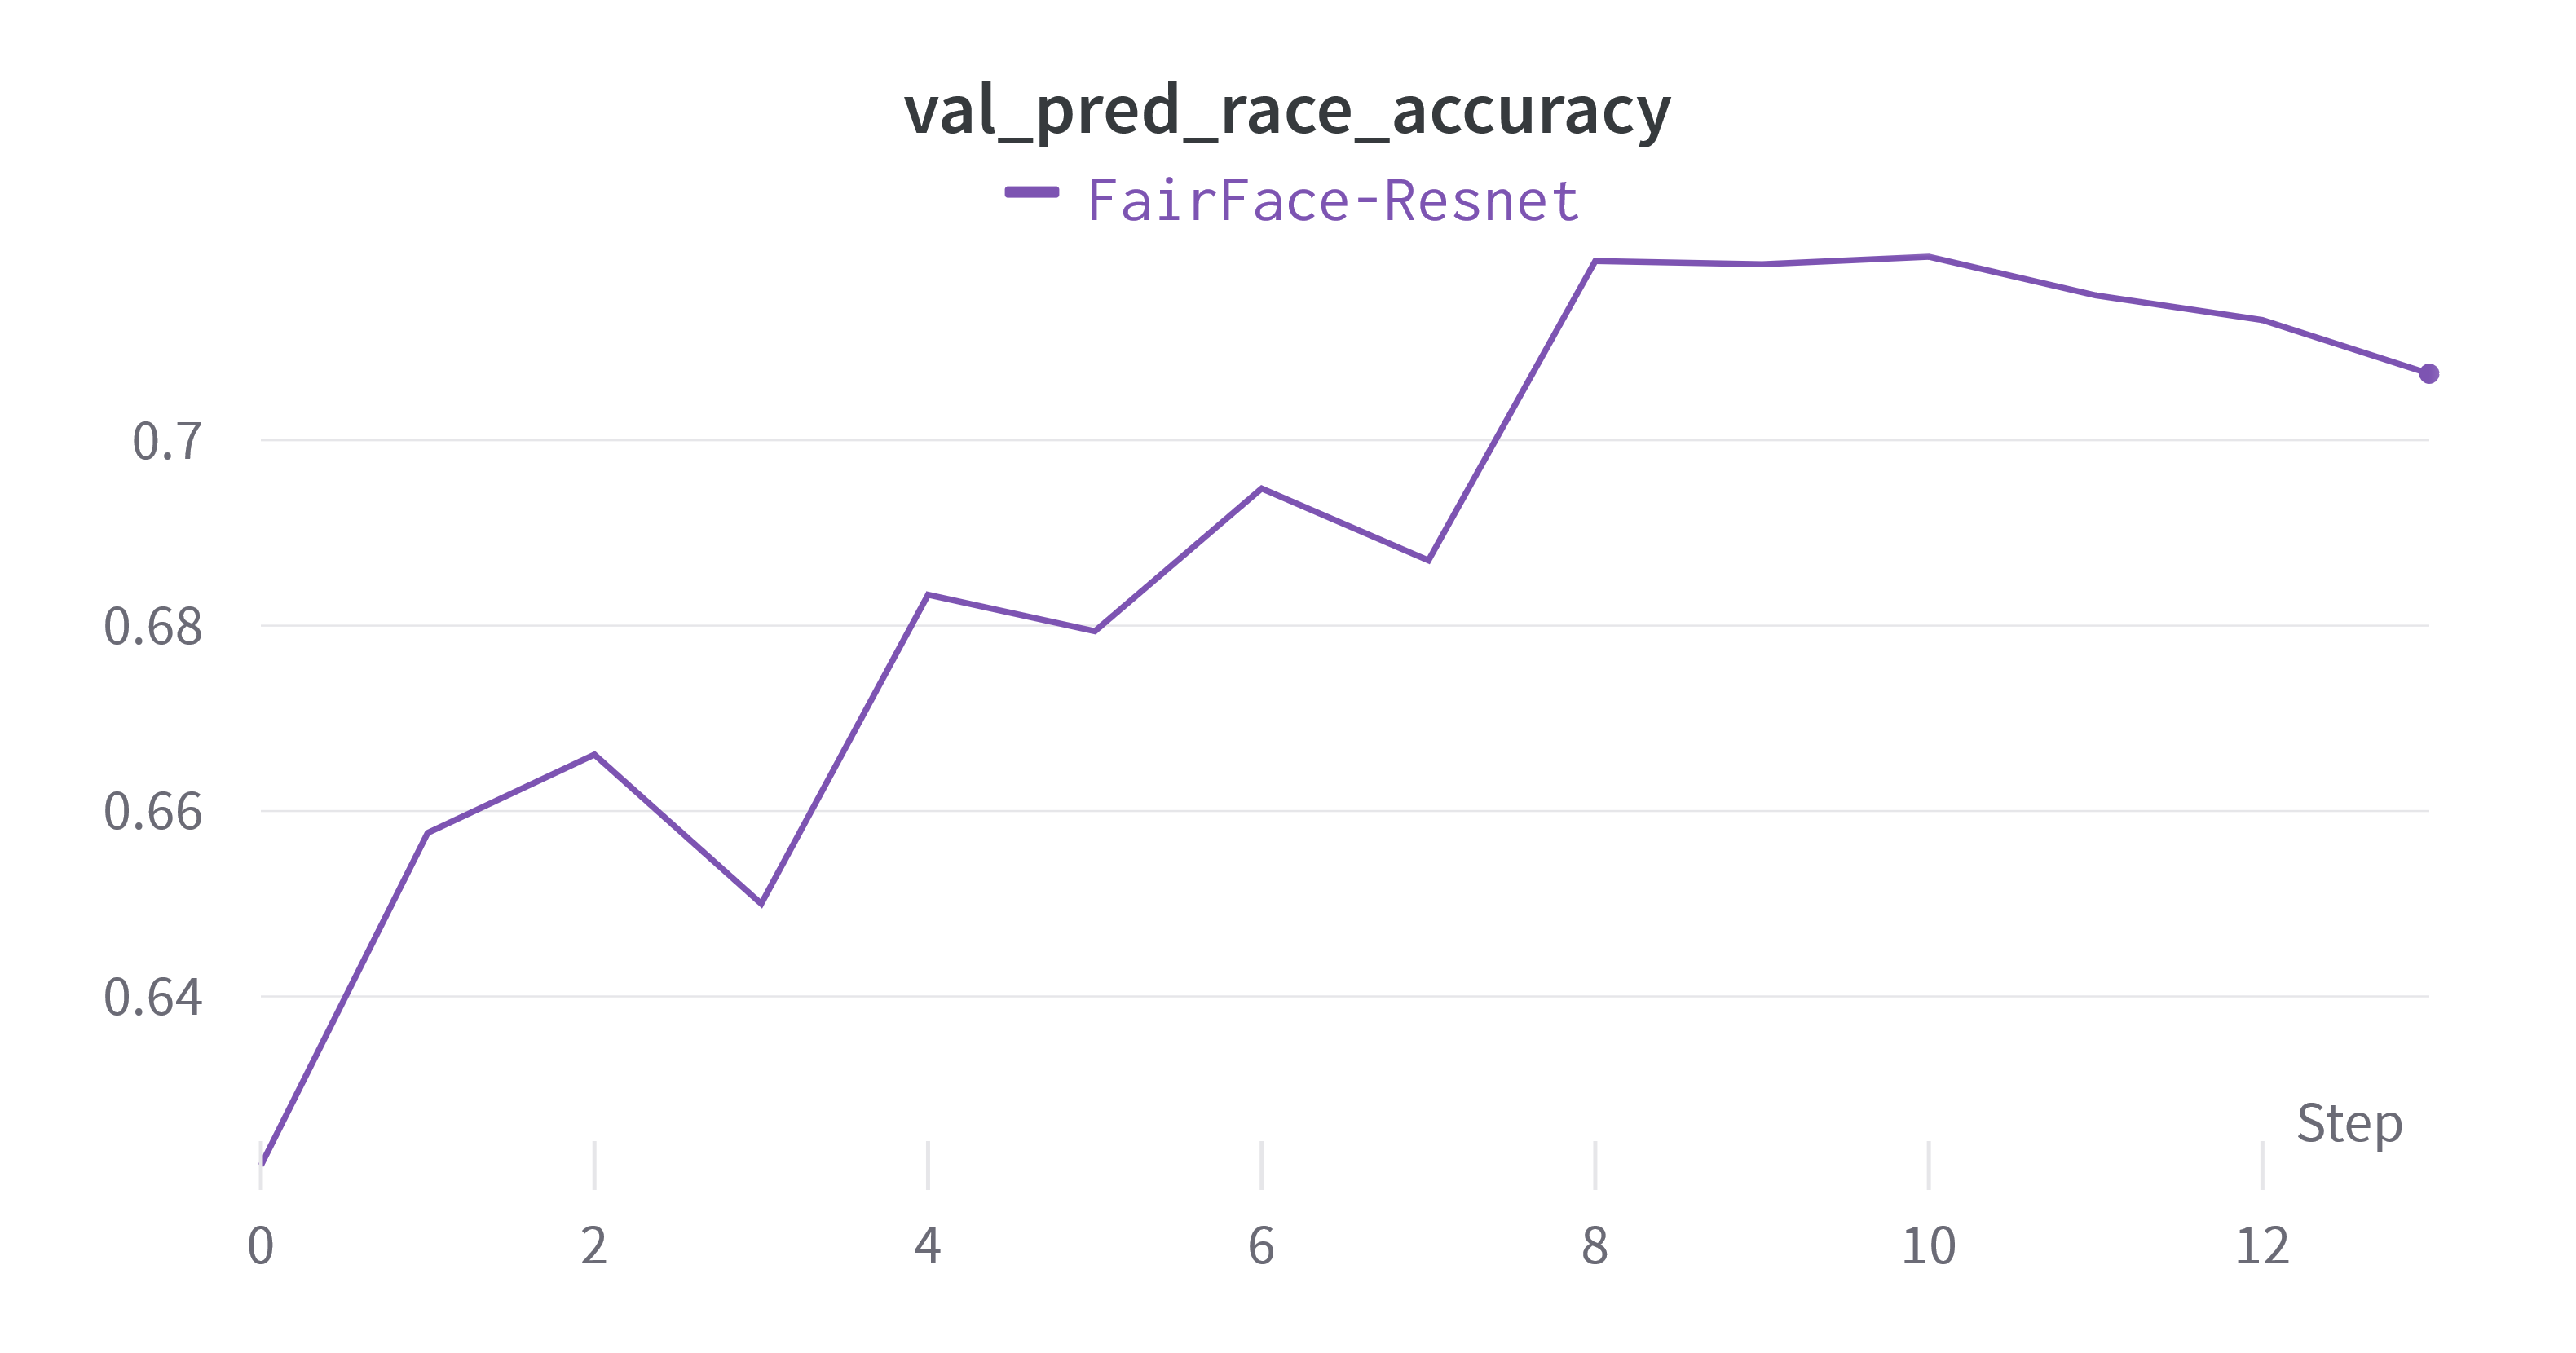
\includegraphics[width=\linewidth]{imgs/FairFace-resnet-race.png}}
		\caption{gender-age-race estimation on UTKface and FairFace}
		\label{gender-age-race}
	\end{figure*}

	\subsection{Race prediction}
	
	\begin{table}[H]
		\centering
		\begin{tabular}{|l|l|l|}
			\hline
			 & ResNet& Xception \\ \hline
			gender loss     & 0.172 & 0.194\\ \hline
			age loss        & 3.026 & 4.312\\ \hline
			race loss       & 0.499 & 0.506\\ \hline
			gender accuracy & 0.935 & 0.895\\ \hline
			age accuracy    & 0.196 & 0.180\\ \hline
			race accuracy   & 0.850 & 0.828\\ \hline
		\end{tabular}
		\caption{Results on UTKface}
	\end{table}

	With the above experiments and analysis, we moved on to solve the gender-age-race ternary classification task. We used Xception and ResNet as the pre-trained model. After adding a new softmax layer as the classification head, the modified models were fine-tuned on UTKface with the race label. We implemented early stopping with patient 5. It took 8 epochs for the model to converge, as displayed in Figure \ref{gender-age-race}, (a) - (c). The results from the best epoch on the validation set are as followed.
	
	The age prediction accuracy seems relatively low, which only achieves 19.6\%. The reason is similar to section \ref{sec:backbone}. Additionally, the UTKface considers a more unbalanced distribution of race, and each race is expected to have different age features. Thus, it might be more difficult for the model to predict the exact age. A more fair way to train the model is to combine some of the age classes into a single larger class. This strategy is applied in FairFace.
	
	With the results above, we further analyzed the prediction accuracy for each individual race group. Firstly, we predicted all the images in the test set and combined the predictions with the ground truth into one dataframe. Then, we split the dataframe into 5 sub-dataframes and calculated the accuracy for each sub-dataframe separately. The result is shown in the following table:
	
	\begin{table}[H]
		\centering
		\begin{tabular}{|l|l|}
			\hline
			\textbf{Race Label} & \textbf{Accuracy} \\ \hline
			White  &  0.392 \\ \hline
			Black  & 0.371 \\ \hline
			Asian  & 0.483 \\ \hline 
			Indian & 0.405 \\ \hline 
			Others & 0.415 \\ \hline 
		\end{tabular}
		\caption{Age prediction accuracy over different races (UTKface)}
	\end{table}

	The highest accuracy is Asian, which achieves 48.3\%, but the lowest is only 37.1\%. The accuracy varies among different race groups, which indicates that the UTKface dataset is unfair for different race groups.
	
	To overcome this problem, we trained the model on FairFace, which has a more balanced dataset in terms of the race label, as mentioned in 4.1. The training process is demonstrated in Figure \ref{gender-age-race}, (d) - (f). Below are the results retrieved from the best epoch on the validation set of Fairface:
	
	\begin{table}[H]
		\centering
		\begin{tabular}{|l|l|l|}
			\hline
			  & ResNet & Xception \\ \hline
			gender loss     & 0.945  & 1.167    \\ \hline
			age loss        & 0.036  & 1.069     \\ \hline
			race loss       & 3.043  & 3.860     \\ \hline
			gender accuracy & 0.916  & 0.905	    \\ \hline
			age accuracy    & 0.551  & 0.501     \\ \hline
			race accuracy   & 0.661  & 0.648    \\ \hline
		\end{tabular}
		\caption{Results on FairFace}
	\end{table}
	
	Applying a similar processing method on the Fairface dataset, we obtained the accuracy for each race group:
	
	\begin{table}[H]
		\centering
		\begin{tabular}{|l|l|}
			\hline
			\textbf{FairFace} & \textbf{accuracy}  \\ \hline 
			East Asian 		 & 0.740 \\ \hline
			Indian           & 0.721 \\ \hline 
			Black            & 0.711 \\ \hline
			White            & 0.719 \\ \hline
			Middle Eastern   & 0.724 \\ \hline
			Latino Hispanic  & 0.728 \\ \hline
			Southeast Asian  & 0.727 \\ \hline
		\end{tabular}
		\caption{Age accuracy over different races (FairFace)}
	\end{table}

	The highest accuracy is East Asian with 74.0\% accuracy. The lowest prediction accuracy is Black with 71.1\% accuracy. The difference between these two is less than 3\%, which is much more balanced than that using UTKface dataset. Consider the importance of fairness in the real world deep learning model application, the FairFace dataset is selected for further discussion.
	
	
	\begin{figure*}[t]
		\centering
		\subcaptionbox{}[.45\linewidth][c]{%
			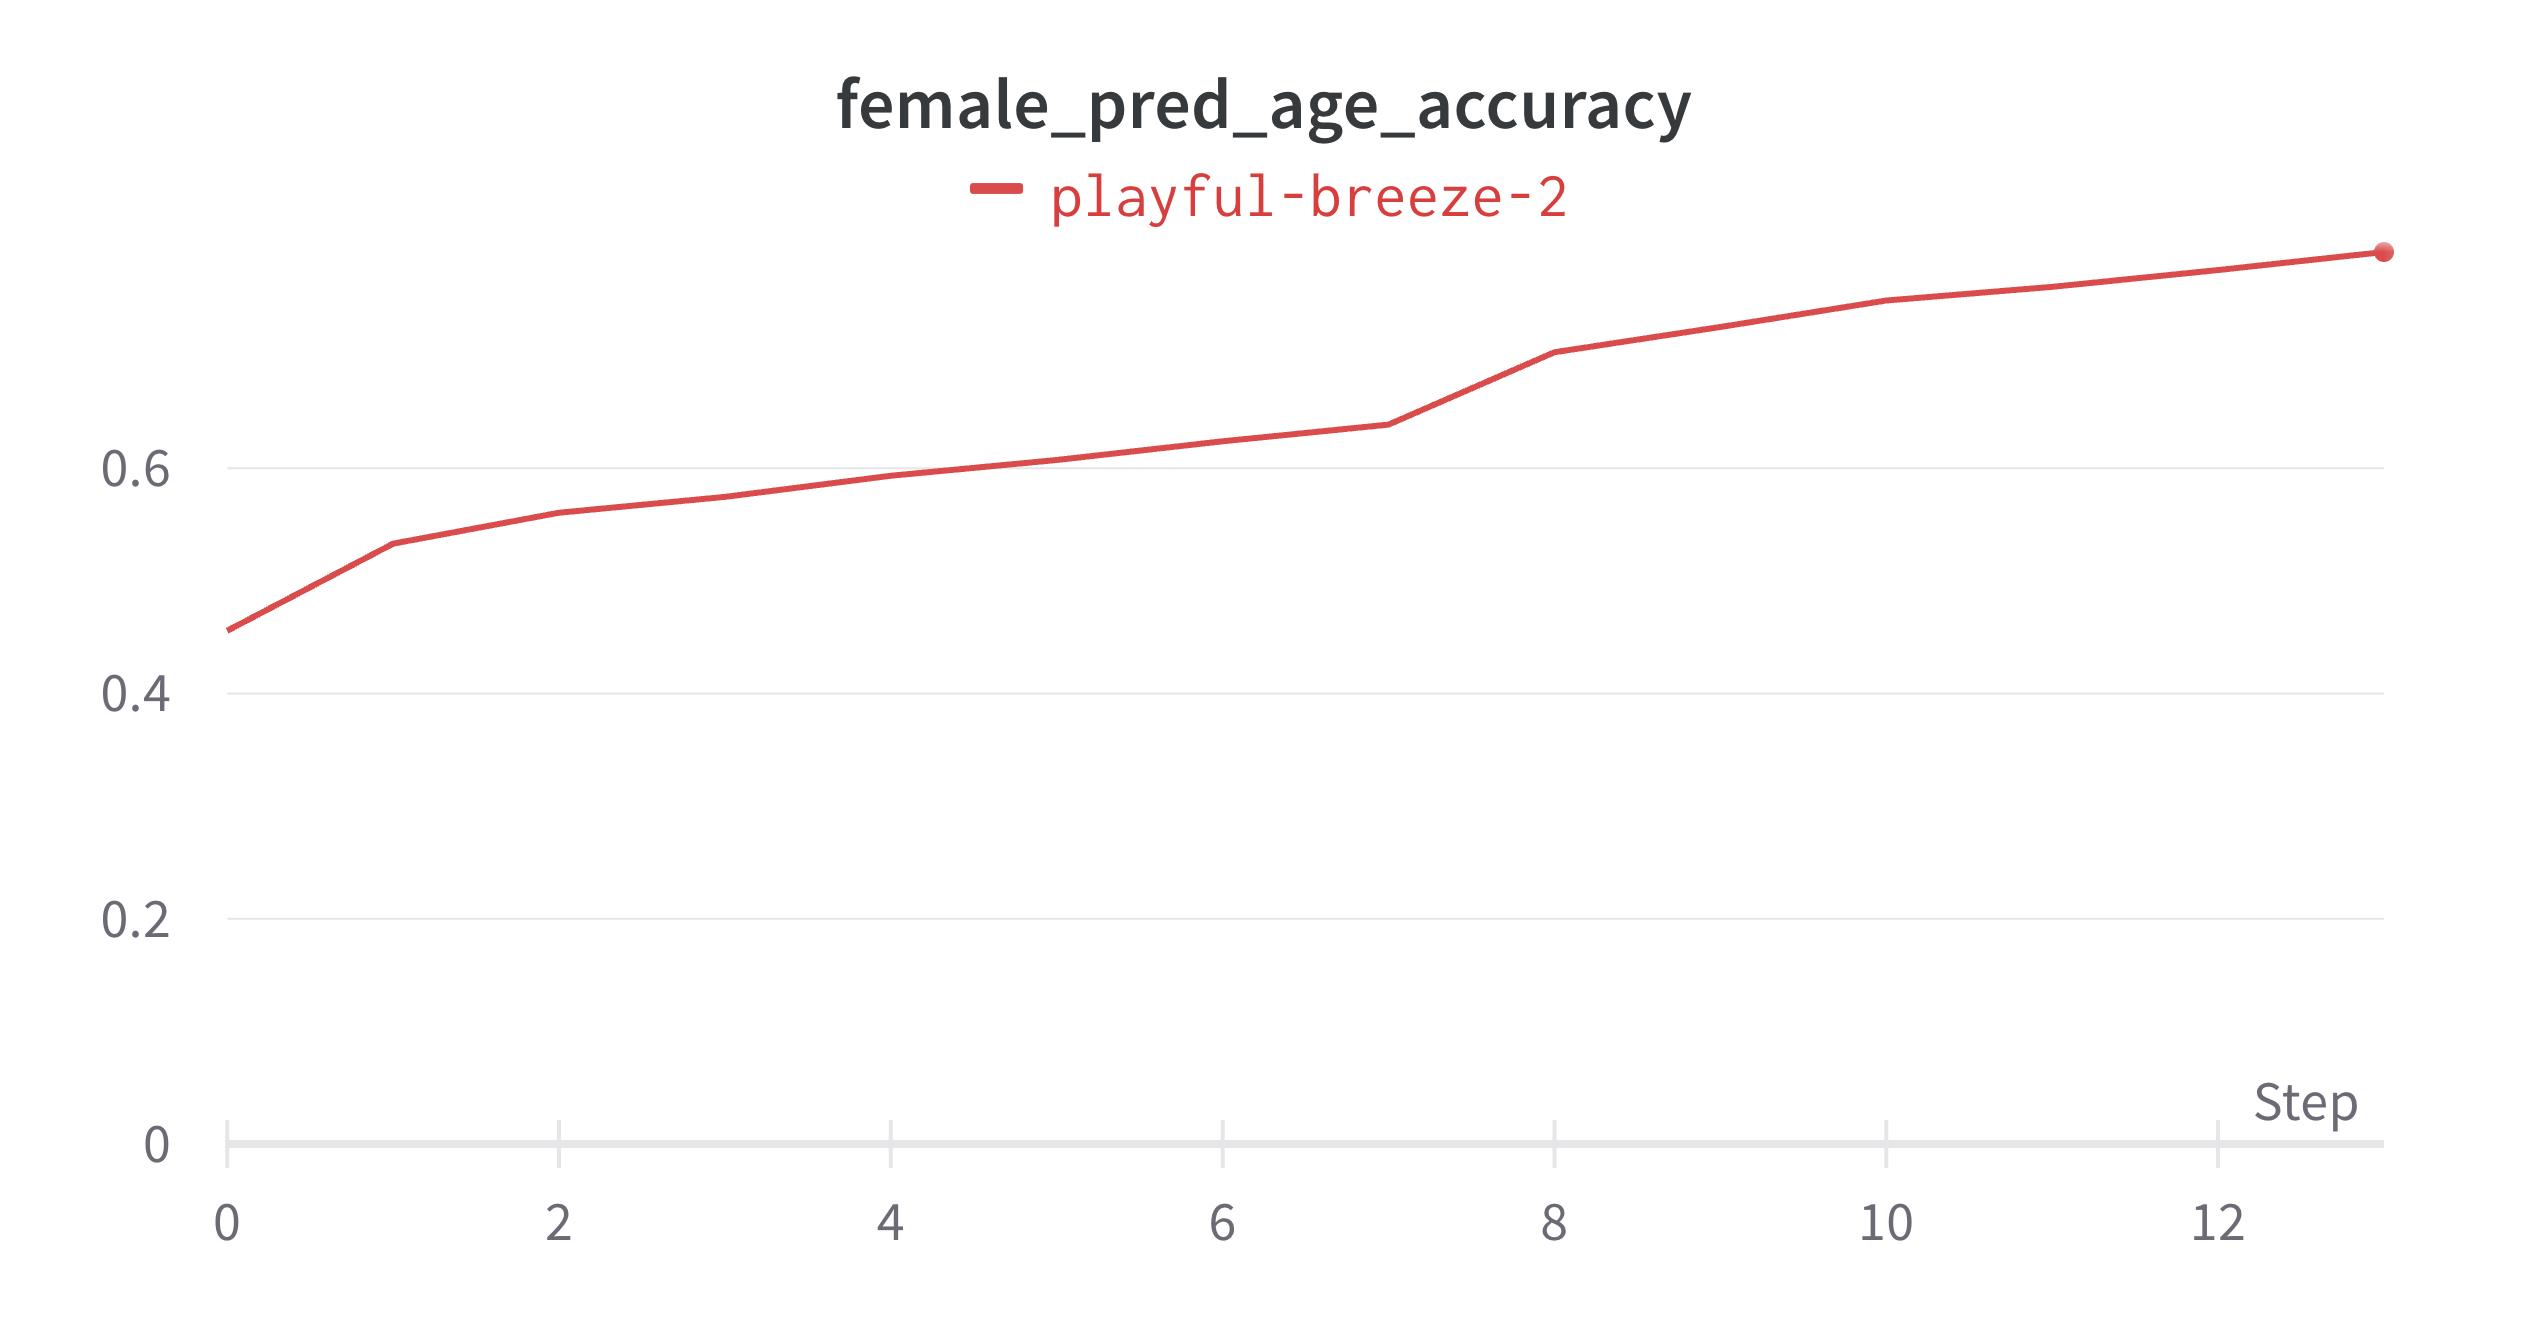
\includegraphics[width=\linewidth]{imgs/female_age.png}}\quad
		\subcaptionbox{}[.45\linewidth][c]{%
			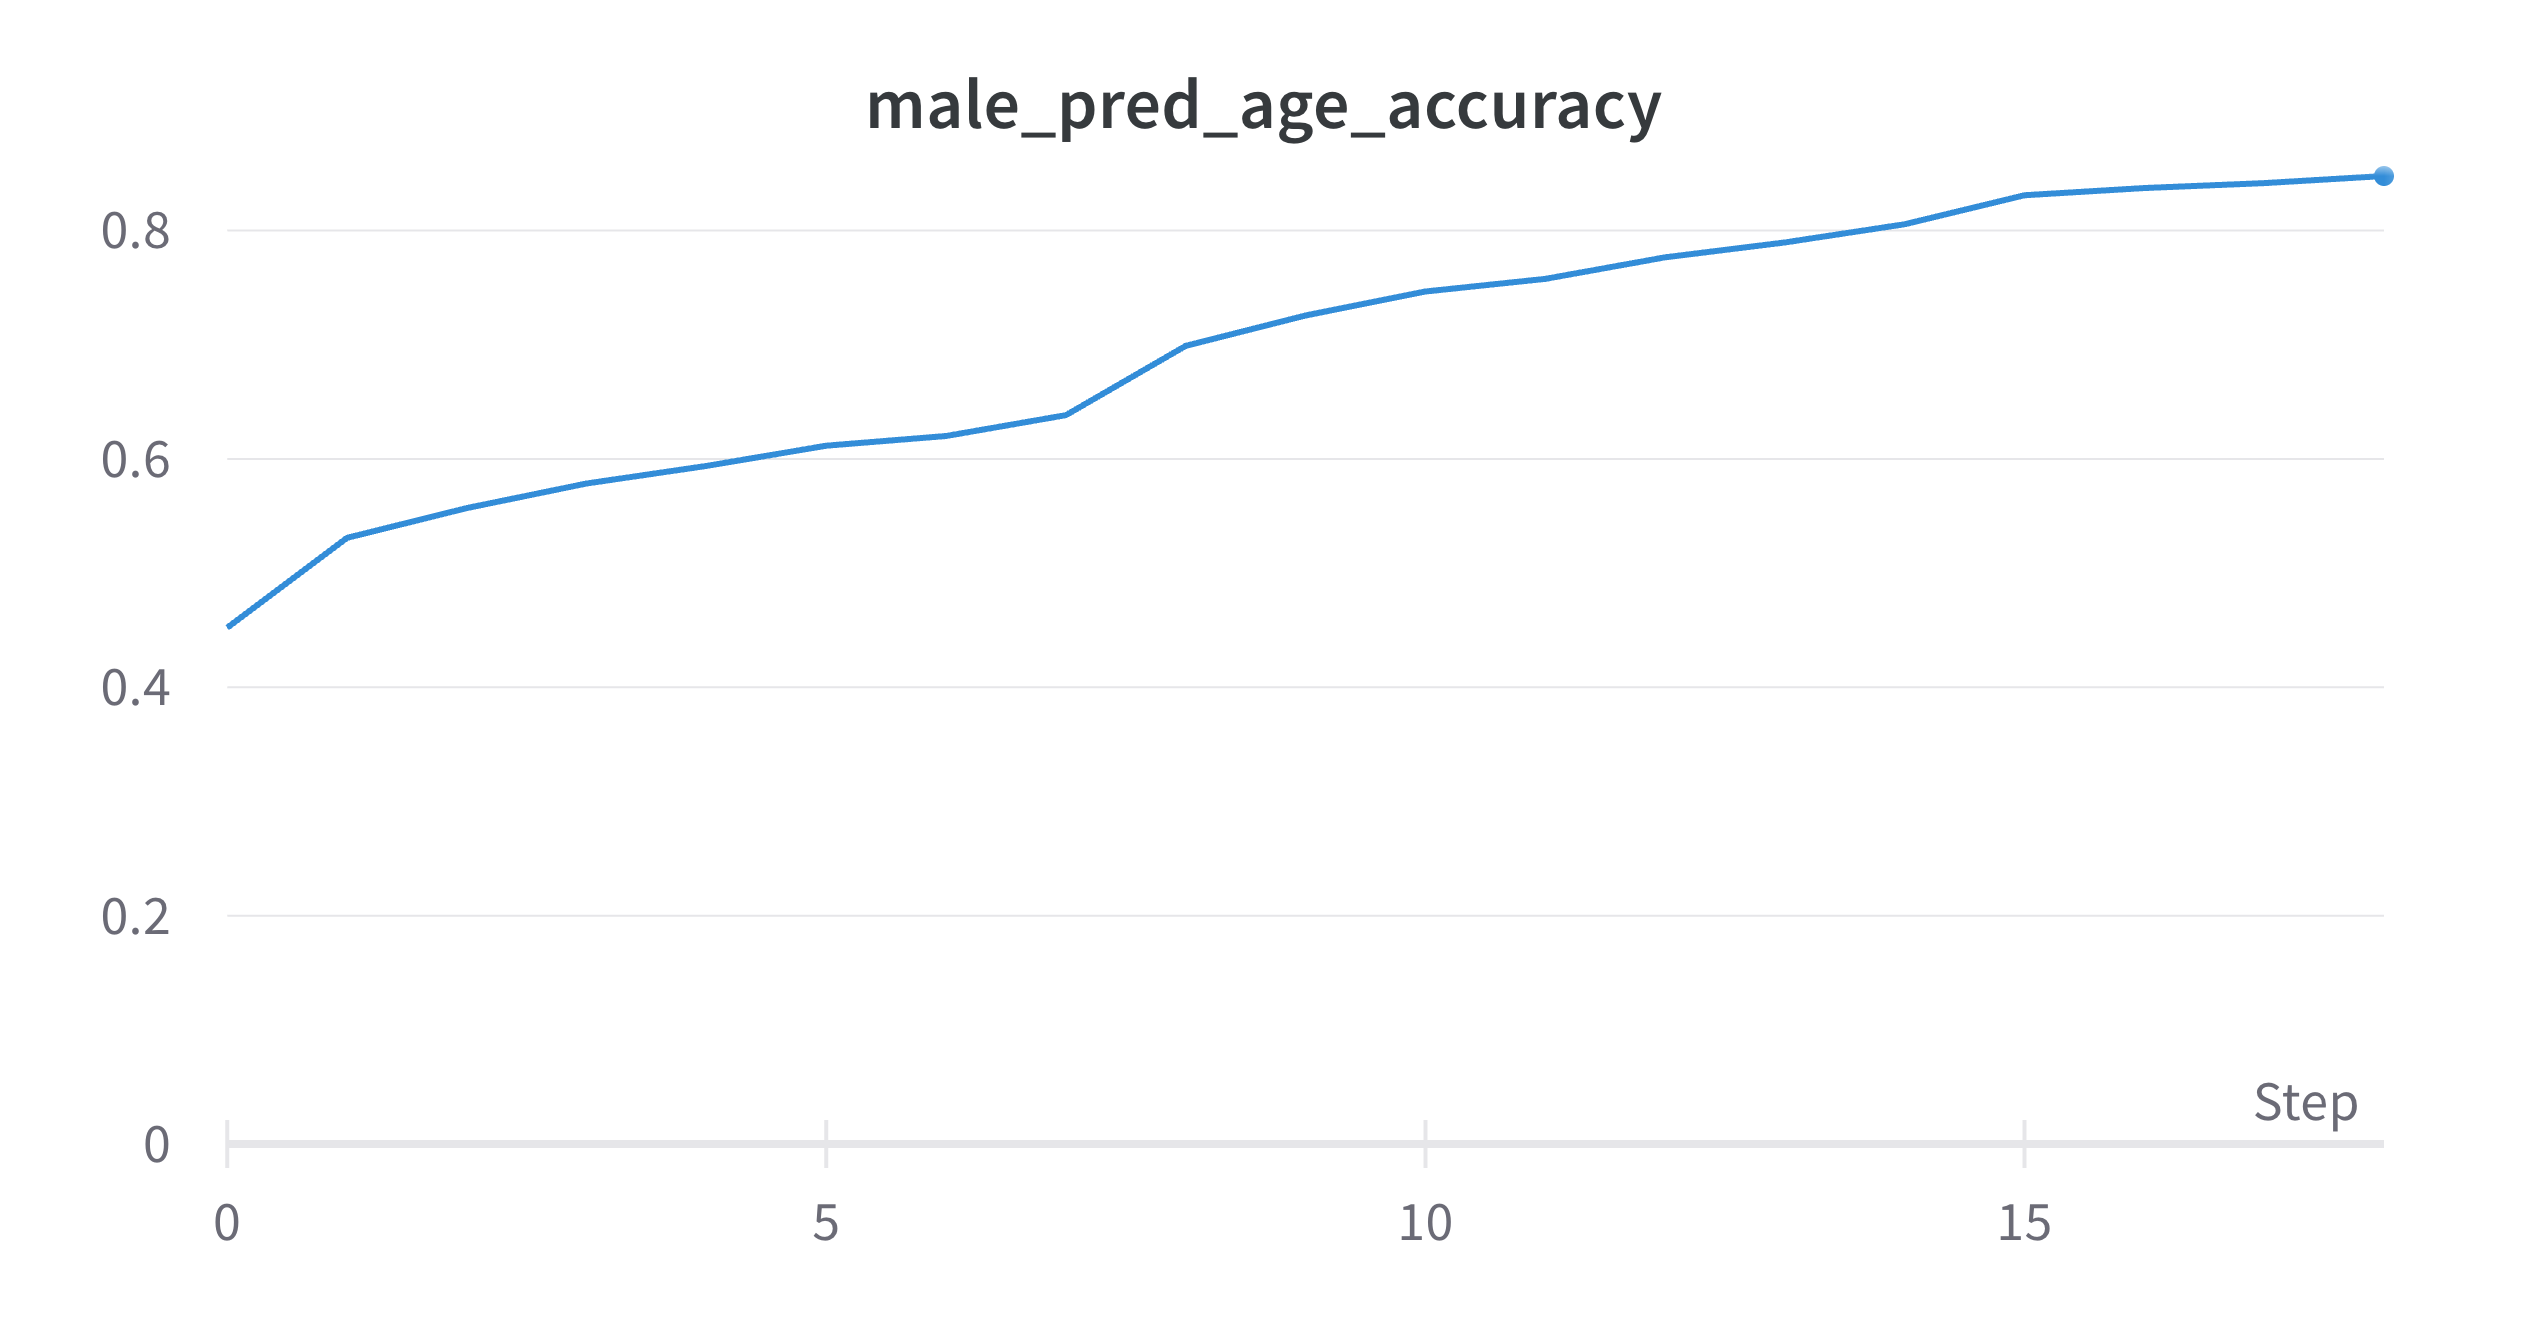
\includegraphics[width=\linewidth]{imgs/male_age.png}}
		\caption{Training of gender-specific age estimation}
		\label{fig:gender_specific_age}
	\end{figure*}
	
	\begin{figure*}[t]
		\centering
		\subcaptionbox{}[.45\linewidth][c]{%
			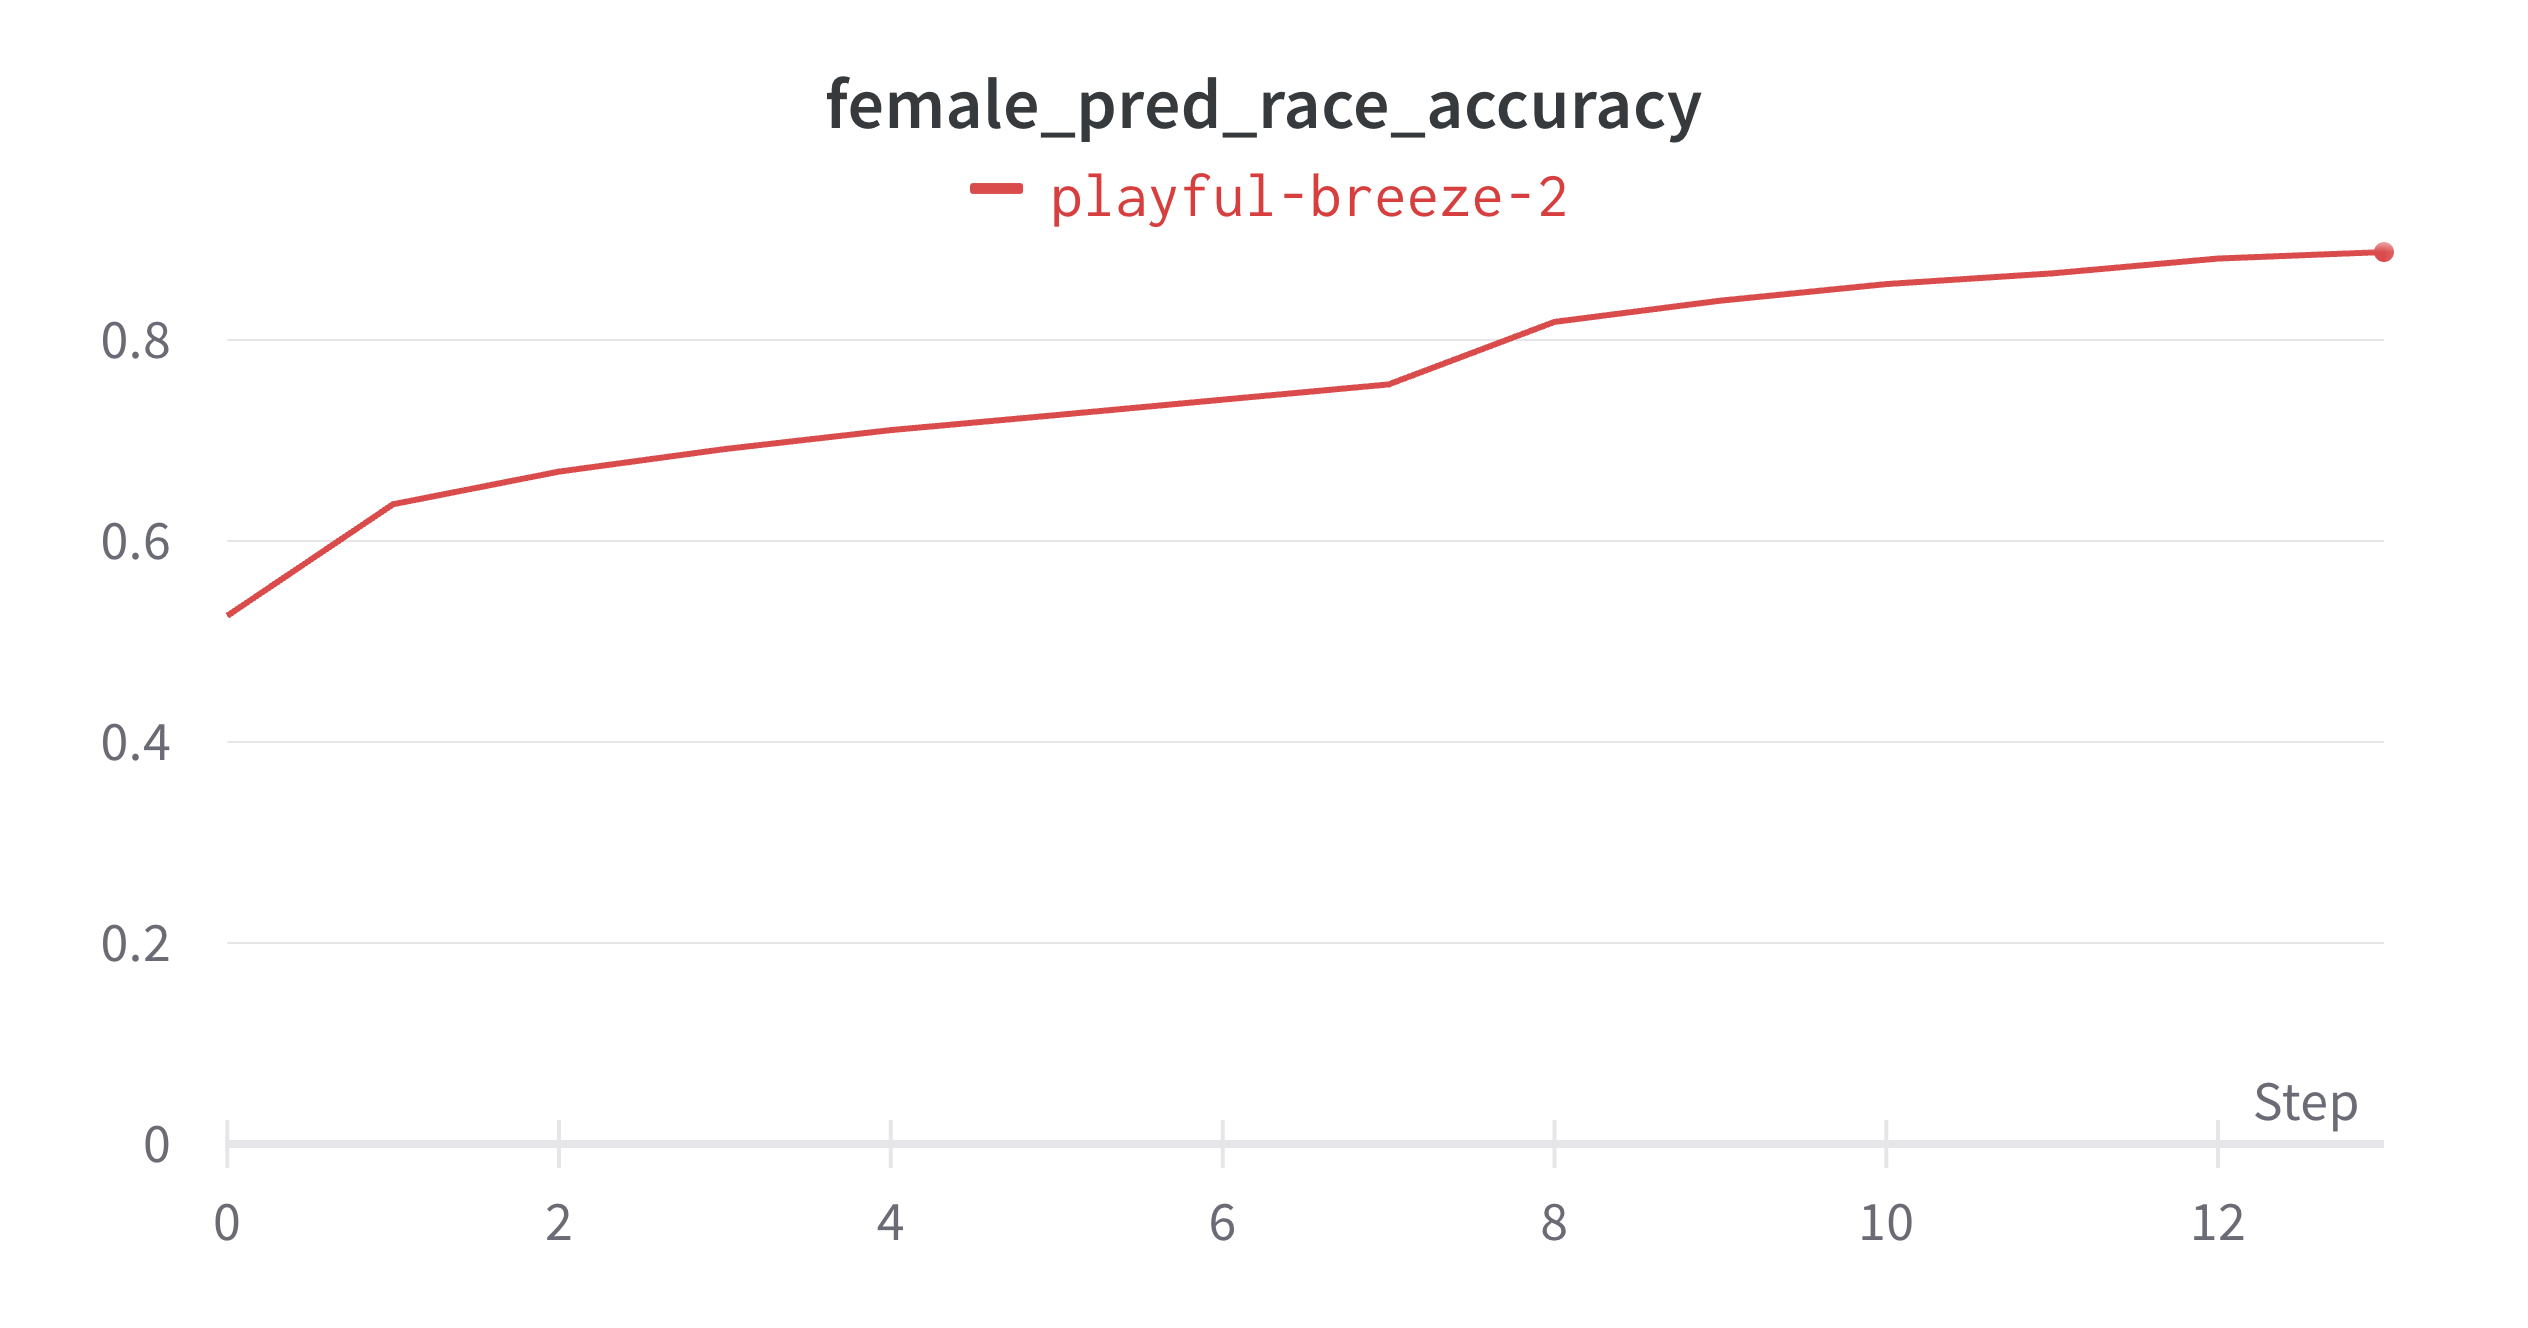
\includegraphics[width=\linewidth]{imgs/female_race.png}}\quad
		\subcaptionbox{}[.45\linewidth][c]{%
			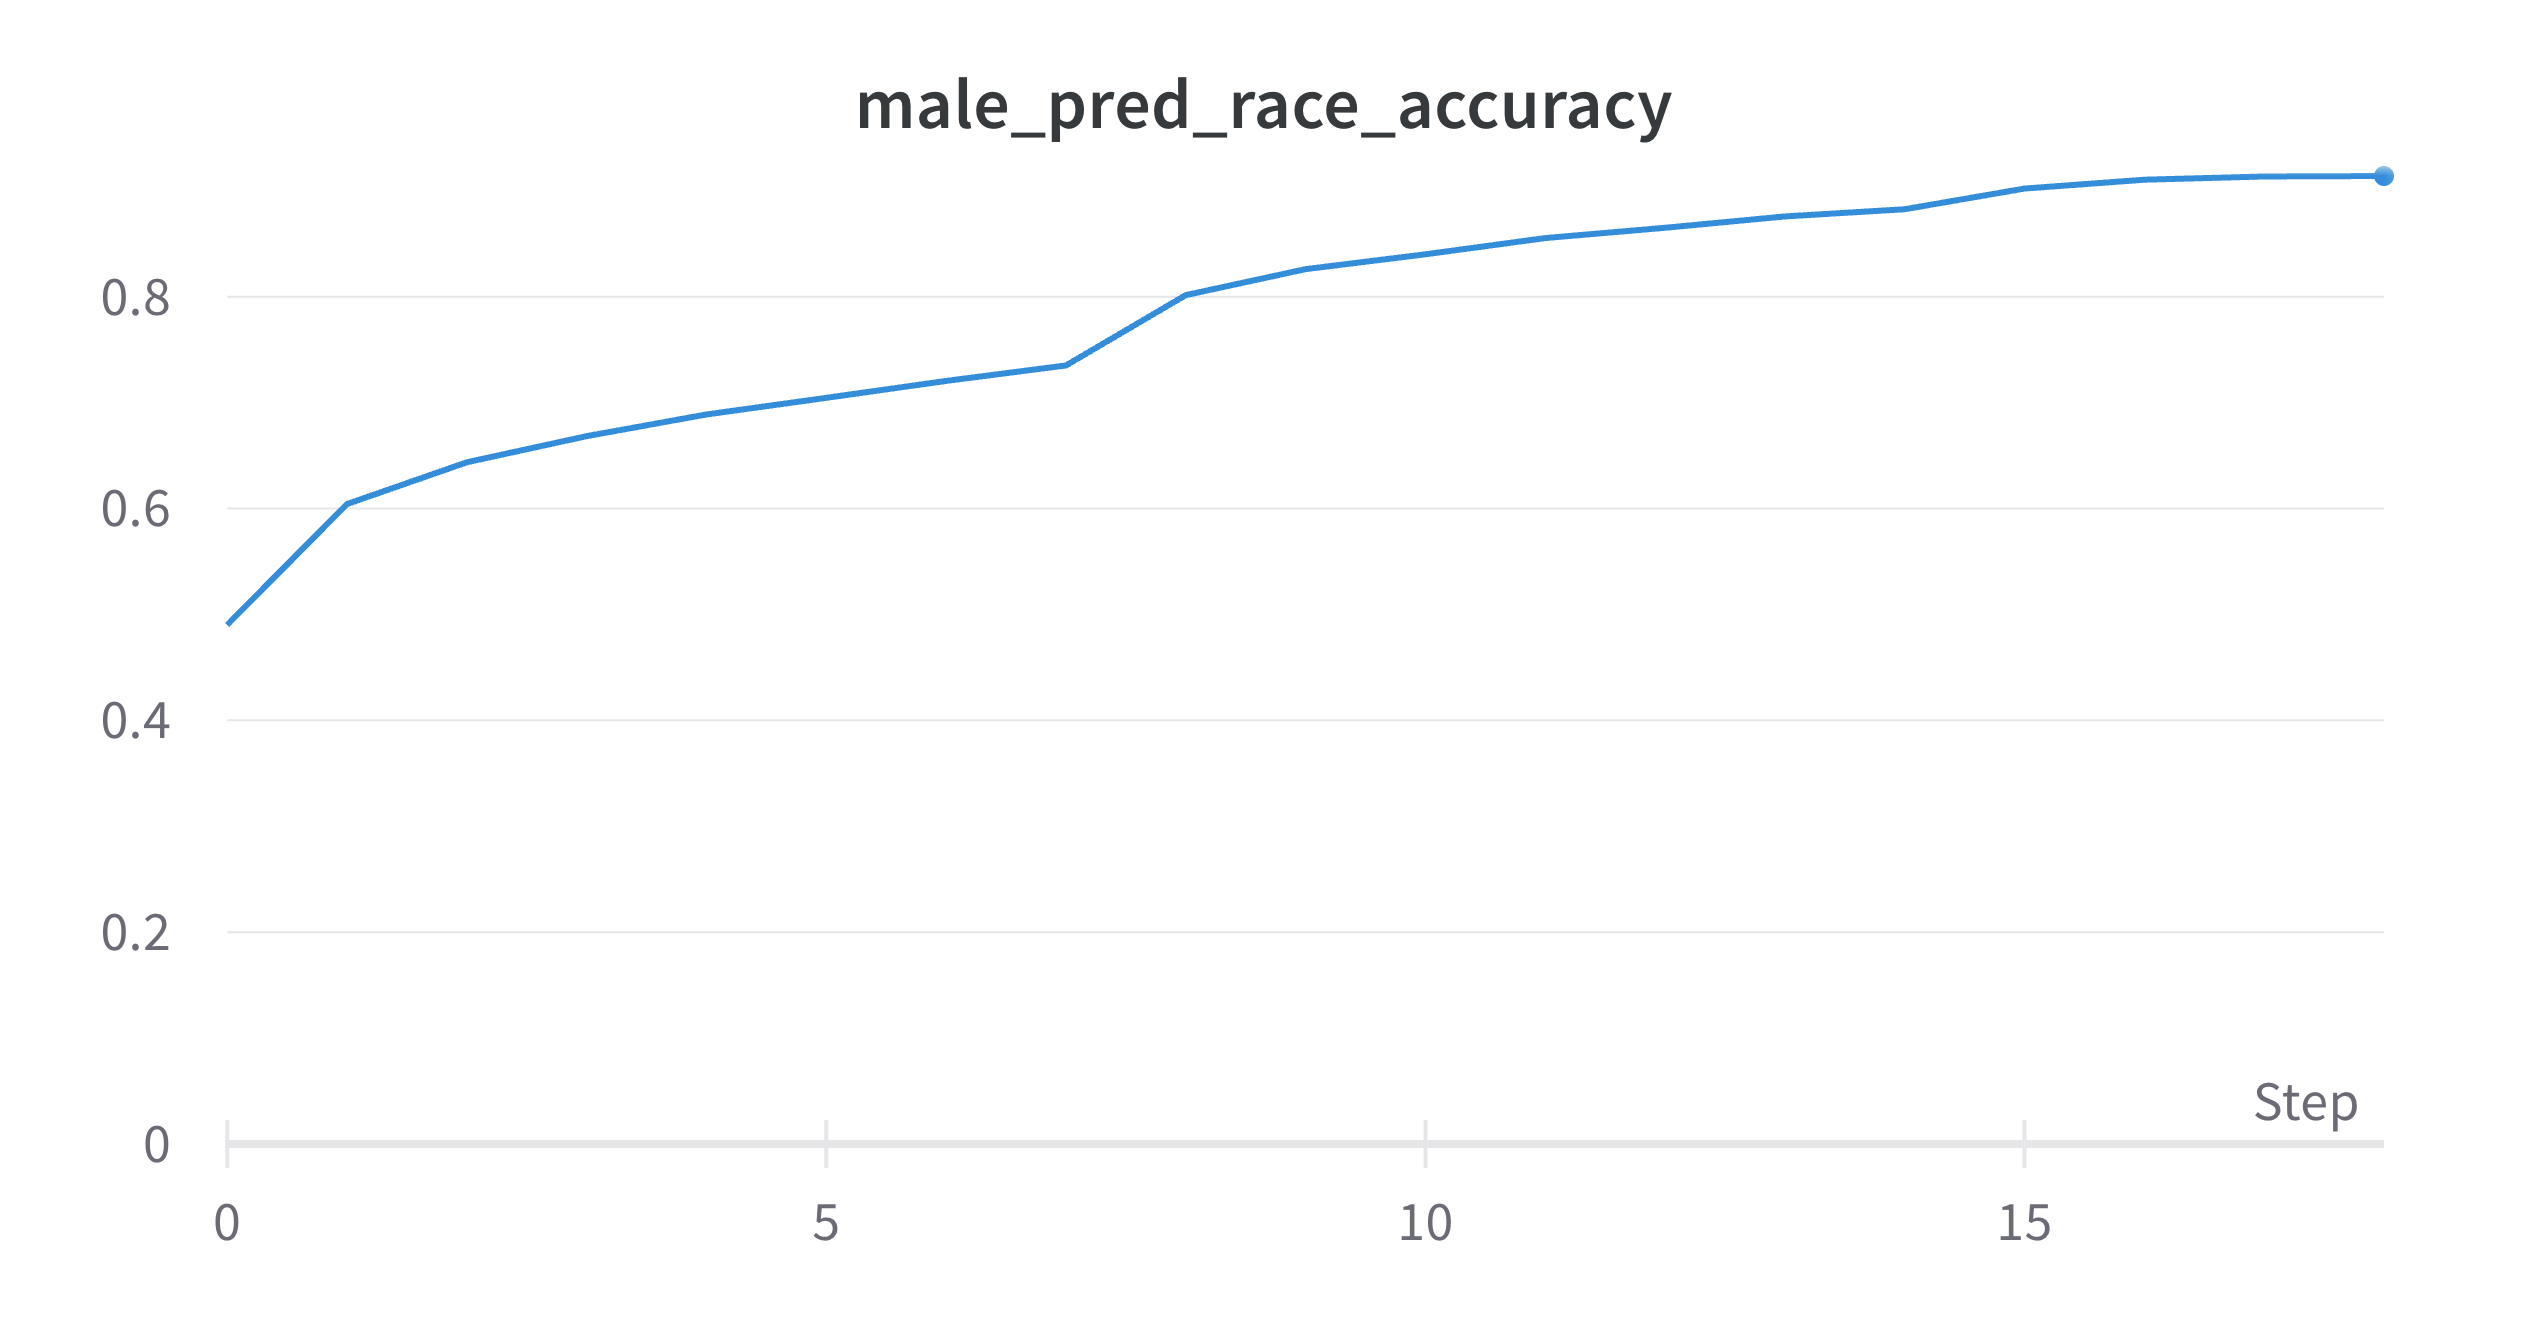
\includegraphics[width=\linewidth]{imgs/male_race.png}}
		\caption{Training of gender-specific race estimation}
		\label{fig:gender_specific_race}
	\end{figure*}

	\subsection{Compare Fusion Model with Original Model}
	
	Our model has a high test accuracy in the task of gender classification. Motivated by this result, we then harnessed the gender-specific information and used this information in the task of age and race estimation. To justify our gender-specific fusion model, we trained the classifiers on each gender separately, and the results are shown in Figure \ref{fig:gender_specific_age} and \ref{fig:gender_specific_race}.
	
	\begin{table}[H]
		\centering
		\begin{tabular}{|l|l|l|}
			\hline
			\textbf{Accuracy} & \textbf{Male} & \textbf{Female}  \\ \hline 
			Age	train	 & 0.848 & 0.792 \\ \hline
			Age val		 & 0.588 & 0.575 \\ \hline
			Race train   & 0.914 & 0.887 \\ \hline 
			Race val     & 0.689 & 0.686 \\ \hline
		\end{tabular}
		\caption{Results on training the classifier separately on male and female images}
	\end{table}
	
	
	The table above also demonstrates the differences more intuitively. We noticed that when training solely on the male images, the accuracy of age and race estimation increased, while the accuracy decreased when training on the female images. This corresponds to our hypothesis that the gender-specific features can affect the training of predictions. There are many differences between the two genders, hence, if we trained two age-and-race classifiers on the male dataset or female dataset separately, the fusion model can learn from its own gender features more effectively. The final test accuracy of the gender-specific model and the original model is shown below. 
	
	\begin{table}[H]
		\centering
		\begin{tabular}{|c|c|c|c|}
			\hline
			Label & Original & Fusion & Improvement \\ 
			\hline
			Gender & 0.916 & 0.935 & +0.019 \\ 
			\hline
			Age & 0.551 & 0.579 & +0.028 \\
			\hline
			Race & 0.661 & 0.698 & +0.037 \\
			\hline
		\end{tabular}
		\caption{Prediction accuracy of fusion model and original model}
	\end{table}

	
	By taking advantage of the gender-specific information, the fusion model achieved an increase of 1.9\% in the accuracy of gender classification, an increase of 2.8\% in the accuracy of age estimation and an increase of 3.7\% in the accuracy of race prediction. Therefore, the fusion model achieved better performance in the gender-age-race classification task. This indicated that given an input image for the age-gender-race classification task, we can first classify its gender, after which put the image into our Male or Female classifier to perform the age and race predictions, and the overall prediction accuracy is higher compared with predicting the three labels altogether using the original model.
	
	We also analyzed some possible reasons for the improvement of our fusion model. Firstly, by training solely on the male and female dataset, our Male and Female classifier might be less distracted by the opposite gender, and hence concentrate more on its own gender-specific features to perform more accurate predictions on age and race. Secondly, with the 2-stage fusion architecture, the overall model can effectively harness the gender-specific information, which is omitted by the original model. This also corresponds to our previous hypothesis. 
	

	
	\section{Discussion} 
	\subsection{Backbone of pre-trained model}
	
	Multiple experiments have been conducted to perform a comprehensive comparison between models with different backbones. The backbones employed include VGG, Xception and ResNet.
	
	\begin{itemize}
		\item The VGG family which includes VGG-16 and VGG-19 \cite{simonyan2014very}, is one of the most famous backbones used for computer vision tasks. TThe VGGs architecture has demonstrated its effectiveness in various tasks, including object detection and image segmentation. Furthermore, the VGG family has also been widely employed in many other architectures as the backbone (for feature extraction) in multiple well-known models like R-CNN,Faster R-CNN, and SSD.
		\item Inception is one of the most widely employed backbones, and it is constructed based on inception blocks. Each inception block is a set of convolution layers, and the filter sizes vary from 1x1, 3x3 to 5x5, which can help the network benefit from a multi-scale learning and reduce computing costs. It is worth noting that Inception uses global average pooling instead of Max-pooling used in VGG. Based on Inception, Xception \cite{chollet2017xception} further extends the architecture where standard Inception modules are replaced by depth-wise separable convolutions.
		\item Different from the previously introduced CNN architectures, Residual Neural Network \cite{he2016deep} (ResNet) introduced the residual network. ResNet or Residual neural networks consist of some skip-connections or recurrent units between convolutional blocks and pooling layers. Moreover, the block are followed by batch normalization layers.
	\end{itemize}
	
	The performance of different backbones varied in our experiments. Firstly, it is observed that networks with VGG backbone is the least stable ones, which is reasonable as its architecture is the simplest among the backbones mentioned, thus it has the lowest capacity against perturbations. Secondly, Xception outperforms ResNet on Wiki and IMDb datasets. Considering that ResNet is deeper than Xception, while the Wiki and IMDb datasets are small, ResNet may overfit, which leads to the performance degradation. 
	
	\begin{figure}[t]
		\centering
		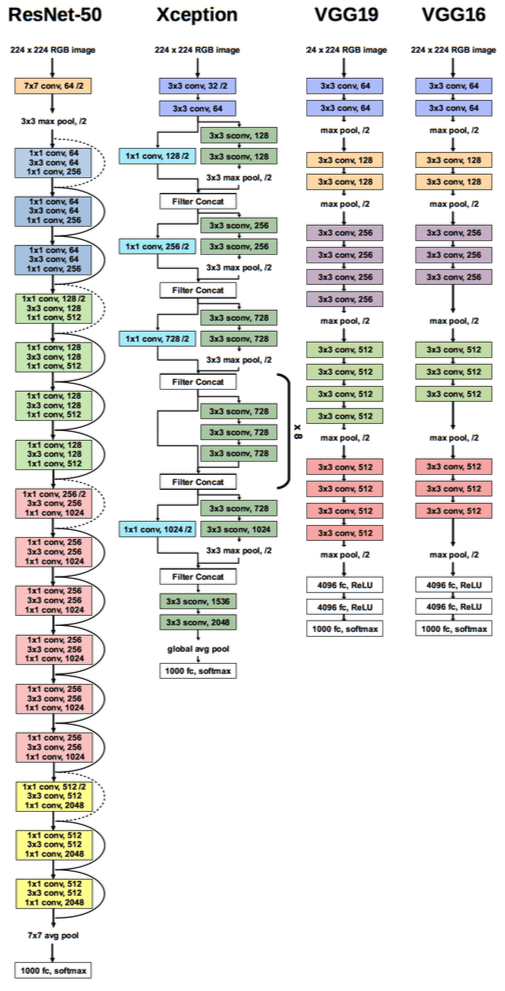
\includegraphics[width=0.9\linewidth]{./imgs/architecture}
		\caption{Architecture comparison among VGG16, VGG19, ResNet-50 and Xception}
		\label{fig:architecture}
	\end{figure}
	
	\subsection{Datasets for model training}
	
	It is observed that dataset selection may have impacts on the trained model performance. As there are more than 100 class labels in the UTKFace dataset for the age classification task, the accuracy is lower than 10\% due to human faces' gradually aging nature. Moreover, even if the model age validation accuracy on IMDb dataset is lower than Wiki dataset, interestingly the model age test accuracy on IMDb dataset is higher than Wiki dataset. As Wiki dataset is relatively smaller than IMDb dataset, It tends to be easier for models to capture image features of the entire validation dataset, thus having a higher validation accuracy. However, when it moves to test datasets, the knowledge obtained from small validation dataset is insufficient for the test dataset, leading to a test accuracy degradation. Furthermore, models trained on imbalanced datasets are more likely to perform poorly, which indicates the importance of using balanced datasets in model training.

	\subsection{Future work}

	The performance of computer vision models heavily relies on the training dataset's quality, while our models are trained on small datasets with heavy augmentation due to the limitation of dataset availability. This may cause model performance degradation as the model cannot capture sufficiently diverse face image patterns. In the future study, we can train both the end-to-end model and the fusion model with larger datasets with richer face image representations, thus the impact of relatively insufficient training samples can be eliminated.

	\section{Conclusion}
	In this report, we first formulated a strong end-to-end baseline by employing the tricks including pre-training and model architecture. With a strong baseline as the foundation, we proposed a 2-stage Gender-specific fusion model to further improve the performance, then discussed about the benefits and drawbacks of employing fusion model design instead of the end-to-end model. Moreover, we discussed about the potential impacts of backbone and dataset selection on model performances, and provided suggestions on methods of performance enhancement besides network architecture design.
	% the bibliography
	\clearpage
	\bibliography{CE4042.bib}
	\bibliographystyle{unsrt}
	
\end{document}